\documentclass[nofilelist]{cslthse-msc}
% to show a list of used packages at the end of the document, delete the nofilelist option
%\documentclass{cslthse-msc} 
\usepackage[utf8]{inputenc}
\usepackage[english]{babel}
\usepackage{amsmath}
%\usepackage{amsfonts}
%%\usepackage{amssymb}
\usepackage{amsthm}
%\usepackage{makeidx}
\usepackage{graphicx}
\usepackage[titletoc, header, page]{appendix}
\usepackage{transparent}

% used to display the used files at the end. Select nofilelist as a package option to disable this
\listfiles % initialize

%\geometry{showframe}
%better like this?
\student{Alexander Sandström}{alexander.h.sandstrom@gmail.com}
%\students{Flavius Gruian}{Flavius.Gruian@cs.lth.se}{Camilla Lekebjer}{Camilla.Lekebjer@cs.lth.se}

\thesisnumber{LU-EIT-EX: 2023} % Magic Number! Do not change unless Birger Swahn asks you to do so!
% default is Master. Uncomment the following for "kandidatarbete"/Bachelor's thesis
%\thesistype{Bachelor}{Kandidatarbete}

%\title{Formatting a Master's Thesis}
\title{Drones for Sea Rescue: A Quality of Experience Study of Camera Control}
\svensktitel{Drönare inom Sjöräddning: en Studie i Operatörsupplevelse av Kamerakontroll}

%\onelinetitle
%\twolinestitle
\threelinestitle
%\fourlinestitle

%\subtitle{A suitable subtitle}
\company{the Swedish Sea Rescue Society and the Department of Electrical and Information Technology, Lund University}
\supervisors{Fredrik Falkman, \href{mailto:fredrik.falkman@ssrs.se}{\texttt{fredrik.falkman@ssrs.se}}}{William Tärneberg, \href{mailto:william.tarneberg@eit.lth.se}{\texttt{william.tarneberg@eit.lth.se}}}
\examiner{Maria Kihl, \href{mailto:maria.kihl@eit.lth.se}{\texttt{maria.kihl@eit.lth.se}}}

\date{\today}
%\date{January 16, 2015}

\acknowledgements{
If you want to thank people, do it here, on a separate right-hand page. Both the U.S. \textit{acknowledgments} and the British \textit{acknowledgements} spellings are acceptable.

}

\theabstract{
Your abstract should capture, in English, the whole thesis with focus on the problem and solution in 150 words. It should be placed on a separate right-hand page, with an additional \textit{1cm} margin on both left and right. Avoid acronyms, footnotes, and references in the abstract if possible.

Leave a \textit{2cm} vertical space after the abstract and provide a few keywords relevant for your report. Use five to six words, of which at most two should be from the title.
}

\keywords{MSc, BSc, template, report, style, structure}

%% Only used to display font sizes
\makeatletter
\newcommand\thefontsize[1]{{#1 \f@size pt\par}}
\makeatother
%%%%%%%%%%

\begin{document}
\renewcommand{\bibname}{References}

\makefrontmatter
\chapter{Introduction}
This chapter will give a short introduction to use cases of UAVs and the work of SSRS along with the motivation and scope for the thesis work.

\section{Drone use}
With the recent advancements in technology, the use of drones has skyrocketed. Most notably they have been used in warfare for surveillance and attack purposes, but in recent years the civilian applications have also increased (SOURCES). Common civilian use cases are in cinematography, agriculture and delivery, and there is also a growing interest in using drones for search and rescue (GET MORE EXAMPLES). 

Historically drones have been limited by the maximum distance it can travel from it's operator, but with advancementes in mobile network technology the use case for drones has grown stronger as they now have a much larger range and can be controlled from anywhere with an internet connection.   

% The thesis work is a collaboration between the Swedish Sea Rescue Society and the Department of Electrical and Information Technology at (+the Faculty of Engineering?) Lund University.
\section{SSRS Needs}
The SSRS has been conducting a research project called Eyes-On-Scene where drones are to be used to give better information to a rescue crew on their way to the scene of the accident. As part of the project a mission control software in which one can manage a fleet of drones and see their video feeds has been implemented. However, the drone camera can only be controlled by a so called region of interest (ROI), which points the camera at a GPS location provided on a map. This is not ideal for the operator, as the act of uploading a new ROI requires a point to be selected on the map which then is uploaded to the drone, forcing a context switch for the operator from the video feed to the map. Instead, the SSRS want to be able to adjust the gimbal angle with direct controls, such as with a joystick or the arrow keys. The SSRS also wants an estimate of the latency between the drone and the operator, which they currently don't know.

\section{Research Motivation}
With the expansion of newer, low-latency network technologies like 5G, the use case for remote control has grown stronger. With everything from connected cars, remote surgery or log lifting, the uses of real-time remote-control are many.  

In the research field of Quality of Experience the user experience of remote control is studied, and common objects of study are the effects of different network parameters like latency, jitter or image quality. Previous QoE research have been on applications like log lifting \cite{industry4.0} and excavation equipment \cite{latency-impact}, and the highly dynamic environment of a drone flying above the sea can make an interesting study object.

With the promise of real-time remote control over 5G, the systems of tomorrow will be heavily reliant on the uptime and latency of the network, making these systems exposed to vulnerabilities should the network experience high contingency or failure. Therefore, Having a system that can operate in a degraded state, i.e. with high latency, is a necessity. Furthermore, when 5G is more widely adopted and stable, Internet Service Providers (ISPs) might offer plans with different latencies, giving the user a choice of how much they want to pay for latency that their particular application needs.  

\section{Scope}
The scope of the thesis work is to develop manual gimbal control using the ArduPilot firmware, running on a flight controller connected to a servo gimbal. This prototype is then to be used as a test bed for a QoE experiment evaluating the effects of latency on the operator's experience and task performance. If time allows the interface will be integrated into the existing software stack of the EOS project, serving as a proof of concept for manual gimbal control during flight.

\chapter{Background}
In this chapter a breif background will be given of the Swedish Sea Rescue Society along with the drone project that this work is a part of. Then, the research field of Quality of Experience will be introduced, along with the related previous work.

\section{Swedish Sea Rescue Society}
As can be read on their website \cite{ssrs}, the Swedish Sea Rescue Society (SSRS) is a non-profit organization that was founded at a conference in Stockholm in 1906 due to Sweden receiving criticism of its' poor sea rescue. Today, it is a foundation with 40 employees and over 143 000 members, and with 2400 volunteers manning their 260 rescue vessels, they carry out around 90\% of all sea rescues in Sweden all year around.

\subsection{Innovation}
As stated in their statutes \cite{ssrs-statues}, the mission of SSRS is not solely to carry out these rescue missions but to also innovate and collaborate in the area of maritime rescue as well as other aiding activities in society as a whole. As a result of this, the drone project that this thesis is a part of has been conceived along with other innovation projects such as foiling rescue boats and improved rescue vehicles \cite{surtsey-innovation}.

\subsection{Drone Project: Eyes On Scene}
This thesis work is part of a project called Eyes-on-Scene, where a task-specific drone and mission control software has been developed to meet the requirements of sea rescue missions. In this section the drone and surrounding system will be briefly described.

The drone uses a fixed wing frame and is designed for two modes: sprinting and loitering, which allows for short response time while also being able to stay in the air for a long time. The only equipment it carries is a single camera gimbal with adjustable roll, pitch and yaw angles. The current system uses a launchpad for takeoff and the idea is that the plane will be able to land on a rescue vessel or in the water, allowing it to be picked up. 

A web interface for mission control has also been developed in the project. Currently, the interface allows flying to and loitering around waypoints given on a map which also displays both other naval and aerial traffic in real time. The map also shows the the regulatoy zones in which one is not allowed to fly, i.e. close to airports or military zones. The interface provides video from the drone camera which is recorded and accessible after the mission.

\section{Quality of Experience}
Quality of Experience is an emerging research field that is concerned with the user's experience in multimedia systems. It is an inherently multidisciplinary field that has close ties to the field of User Experience (UX) and Human-Computer Interaction (HCI). QoE is also closely related to the field of Quality of Service (QoS), which is concerned with the technical aspects of a system, but aims instead at evaluating the subjective experience through user experiments rather than qualitative measurements.

In the white paper \cite{qoe-definition}, Brunström et al. make a working definition of Quality of Experience: 

\begin{quote}
   \textit{Quality of Experience (QoE) is the degree of delight or annoyance of the user of an application or service. It results from the fulfillment of his or her expectations with respect to the utility and / or enjoyment of the application or service in the light of the user’s personality and current state.} 
\end{quote}


\section{Previous Work}

W. Tärneberg et al. \cite{industry4.0} present a QoE study with industrial equipment on an excavation site where experienced operators controlled their usual equipment remotely at different latencies. 

K. Brunnström et al. \cite{latency-impact} performed a study on log lifting using a head-mounted display system. In the study, latency is introduced both in the display's response to movement as well as the controls. The display delay was found to have a strong effect on nausea, but an observable effect on controller latency could only be found at latencies above 800 ms. 

As part of the Eyes-On-Scene-project, a study was performed at Chalmers by Grote et al. \cite{eos-maritime} where the same emergency call was performed with and without images from a UAV at the emergency site. The study showed that imagery from the accident gave the rescue personnel a sence of control before arriving at the scene when knowing what they were going to face. The crew was also faster at locating a person or object when having aerial footage of the scene.

\chapter{Test Bed for QoE Experiment}
This chapter will go through the technical details of the test bed used in the experiment. First, the hardware provided by SSRS will be presented. Then, the different software packages and APIs will be outlined. Lastly, the software implemented specifically for the test bed and the hoverboard will be introduced.

\section{Hardware}
\begin{description}
   \item[Flight Controller: Pixracer R15] The flight controller is the brain of the aircraft and houses components and connectors relevant to in-flight operations such as servos for control surfaces, GPS and accelorometer. The components and connectors relevant to this thesis has been the serial connector to the Raspberry Pi and the servo-connectors for gimbal.

   \item[Companion Computer: Raspberry Pi 4] The Raspberry Pi serves as the onboard computer, commonly known as the "companion computer" in the context of drone hardware. It is connected to the flight controller via USB and makes it possible to relay messages sent over ethernet instead of radio, allowing to connect to a ground station over the Internet. 

   \item[Gimbal] The gimbal used in the experiment is designed and manufactured by Fredrik Falkman at the SSRS. It is a 3D-printed design that has three degrees of freedom made possible by three servos connected to drive belts that control each axis of the camera. The servos are connected to the flight controller which also provides them with power. When mounted the servo-housing is inside the aircraft while the part with the mounting plate for the camera module sticks out on the bottom of the drone. In \ref{fig:gimbal-pics} the schematics of the gimbal can be seen. 
   
   \begin{figure}[htp]
      \centering
      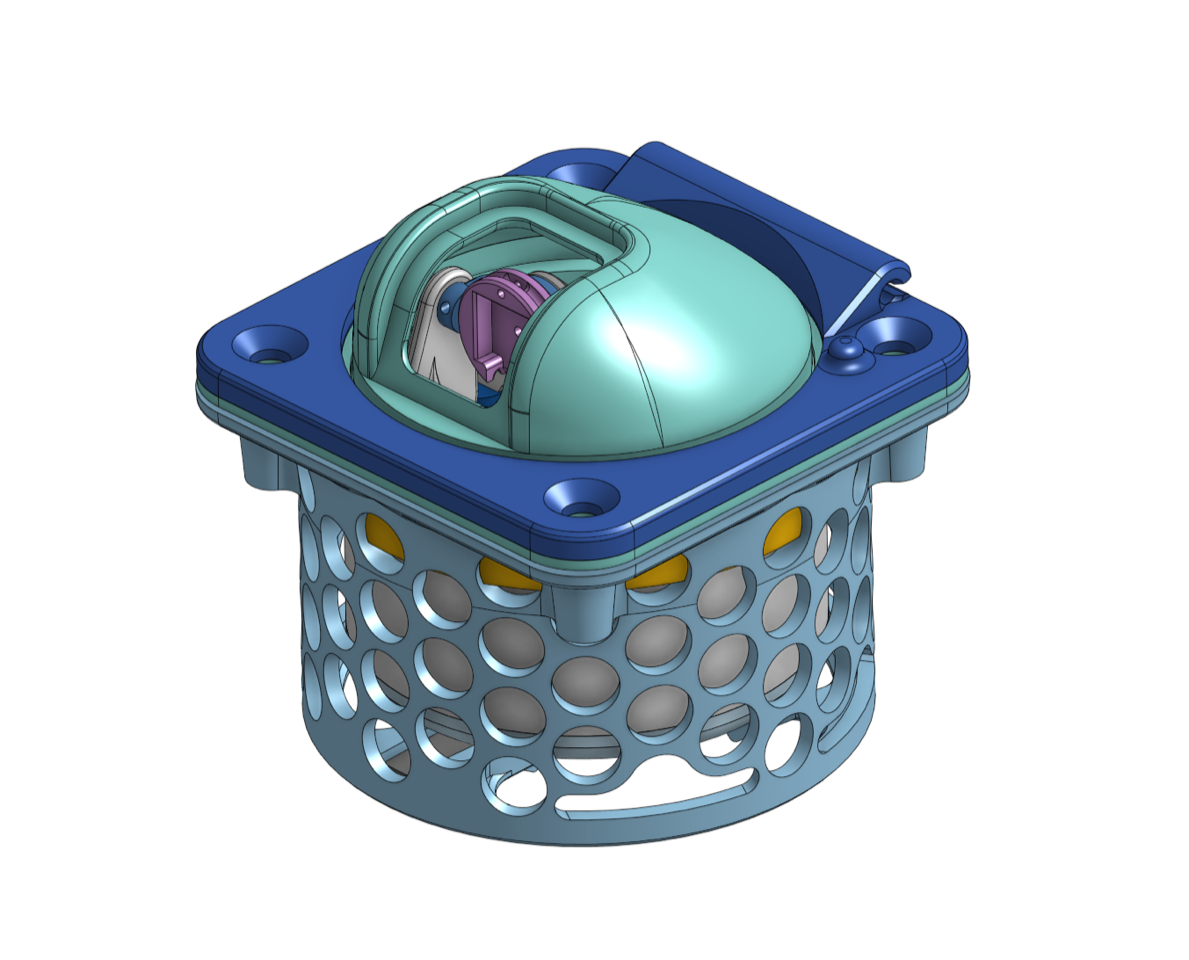
\includegraphics[width=.3\textwidth]{images/gimbal-1.png}\hfill
      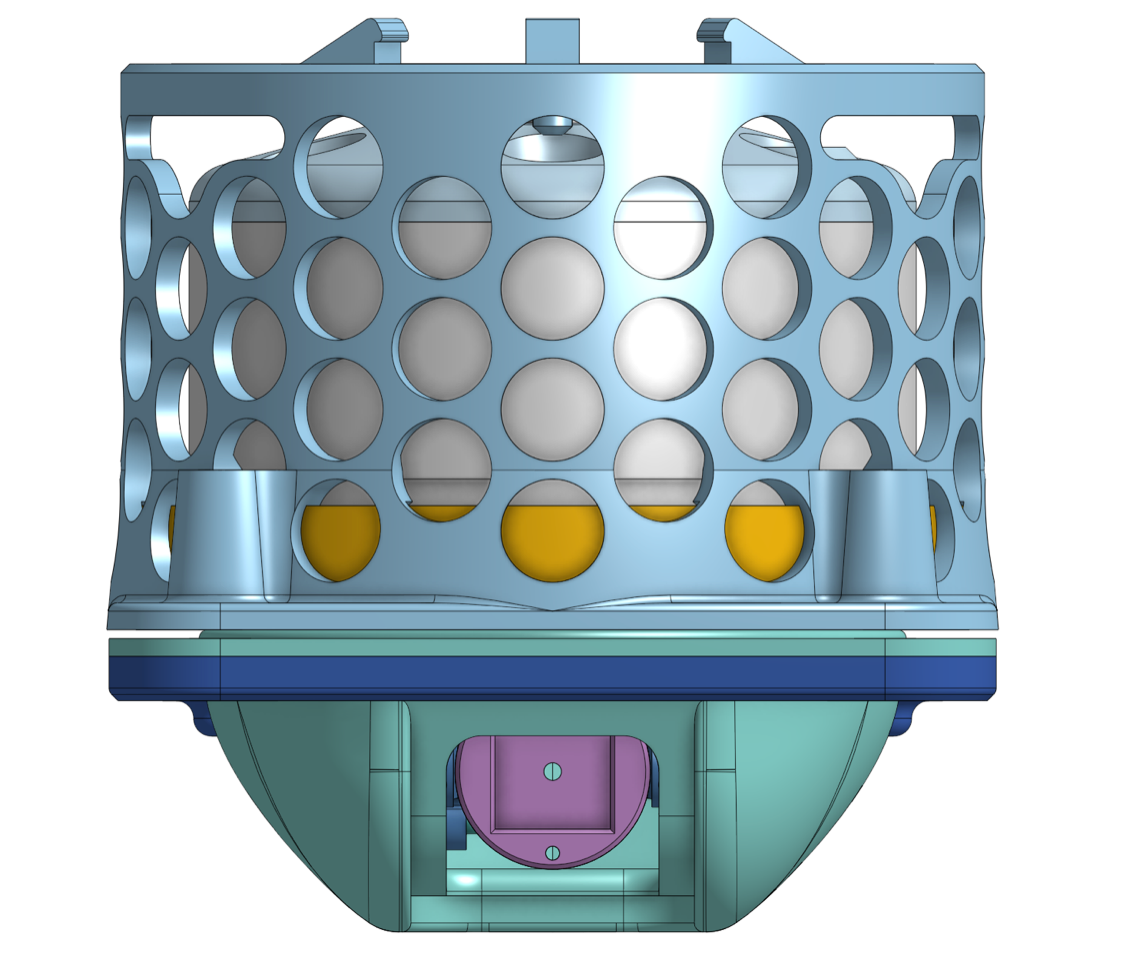
\includegraphics[width=.3\textwidth]{images/gimbal-2.png}\hfill
      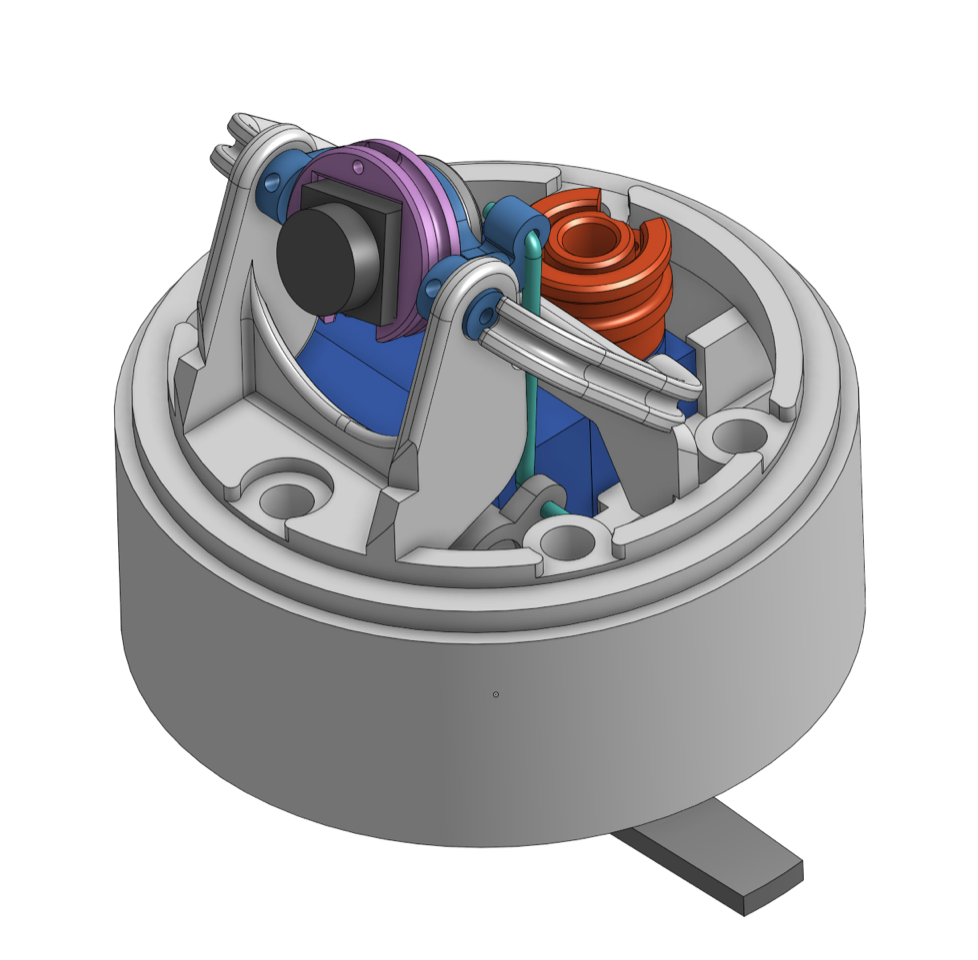
\includegraphics[width=.3\textwidth]{images/gimbal-3.png}
      \caption{Schematics of the gimbal used in the experiment. The middle and left picture shows the gimbal with its full housing. To the right the housing has has been removed and a mockup camera module has been inserted in the mounting plate.}
      \label{fig:gimbal-pics}
   \end{figure}
   
   \item[Raspberry Pi Camera Module v2] The camera module is a small camera that is mounted inside on a flat surface on the gimbal. The camera connects to the module board which is then connected to the Raspberry Pi with a ribbon cable. It is capable of recording 1440x1080 video at 30 fps and has a 4:3 aspect ration.

\end{description}

In the test bed all the components are mounted inside an 2L Ikea SmartStore box where the gimbal is mounted in a cutout in the bottom of the box. The other components are mounted inside the box with velcro tape. Pictures of the box can be seen in figure \ref{fig:drone-setup}. 

\begin{figure}[htp]
   \centering
   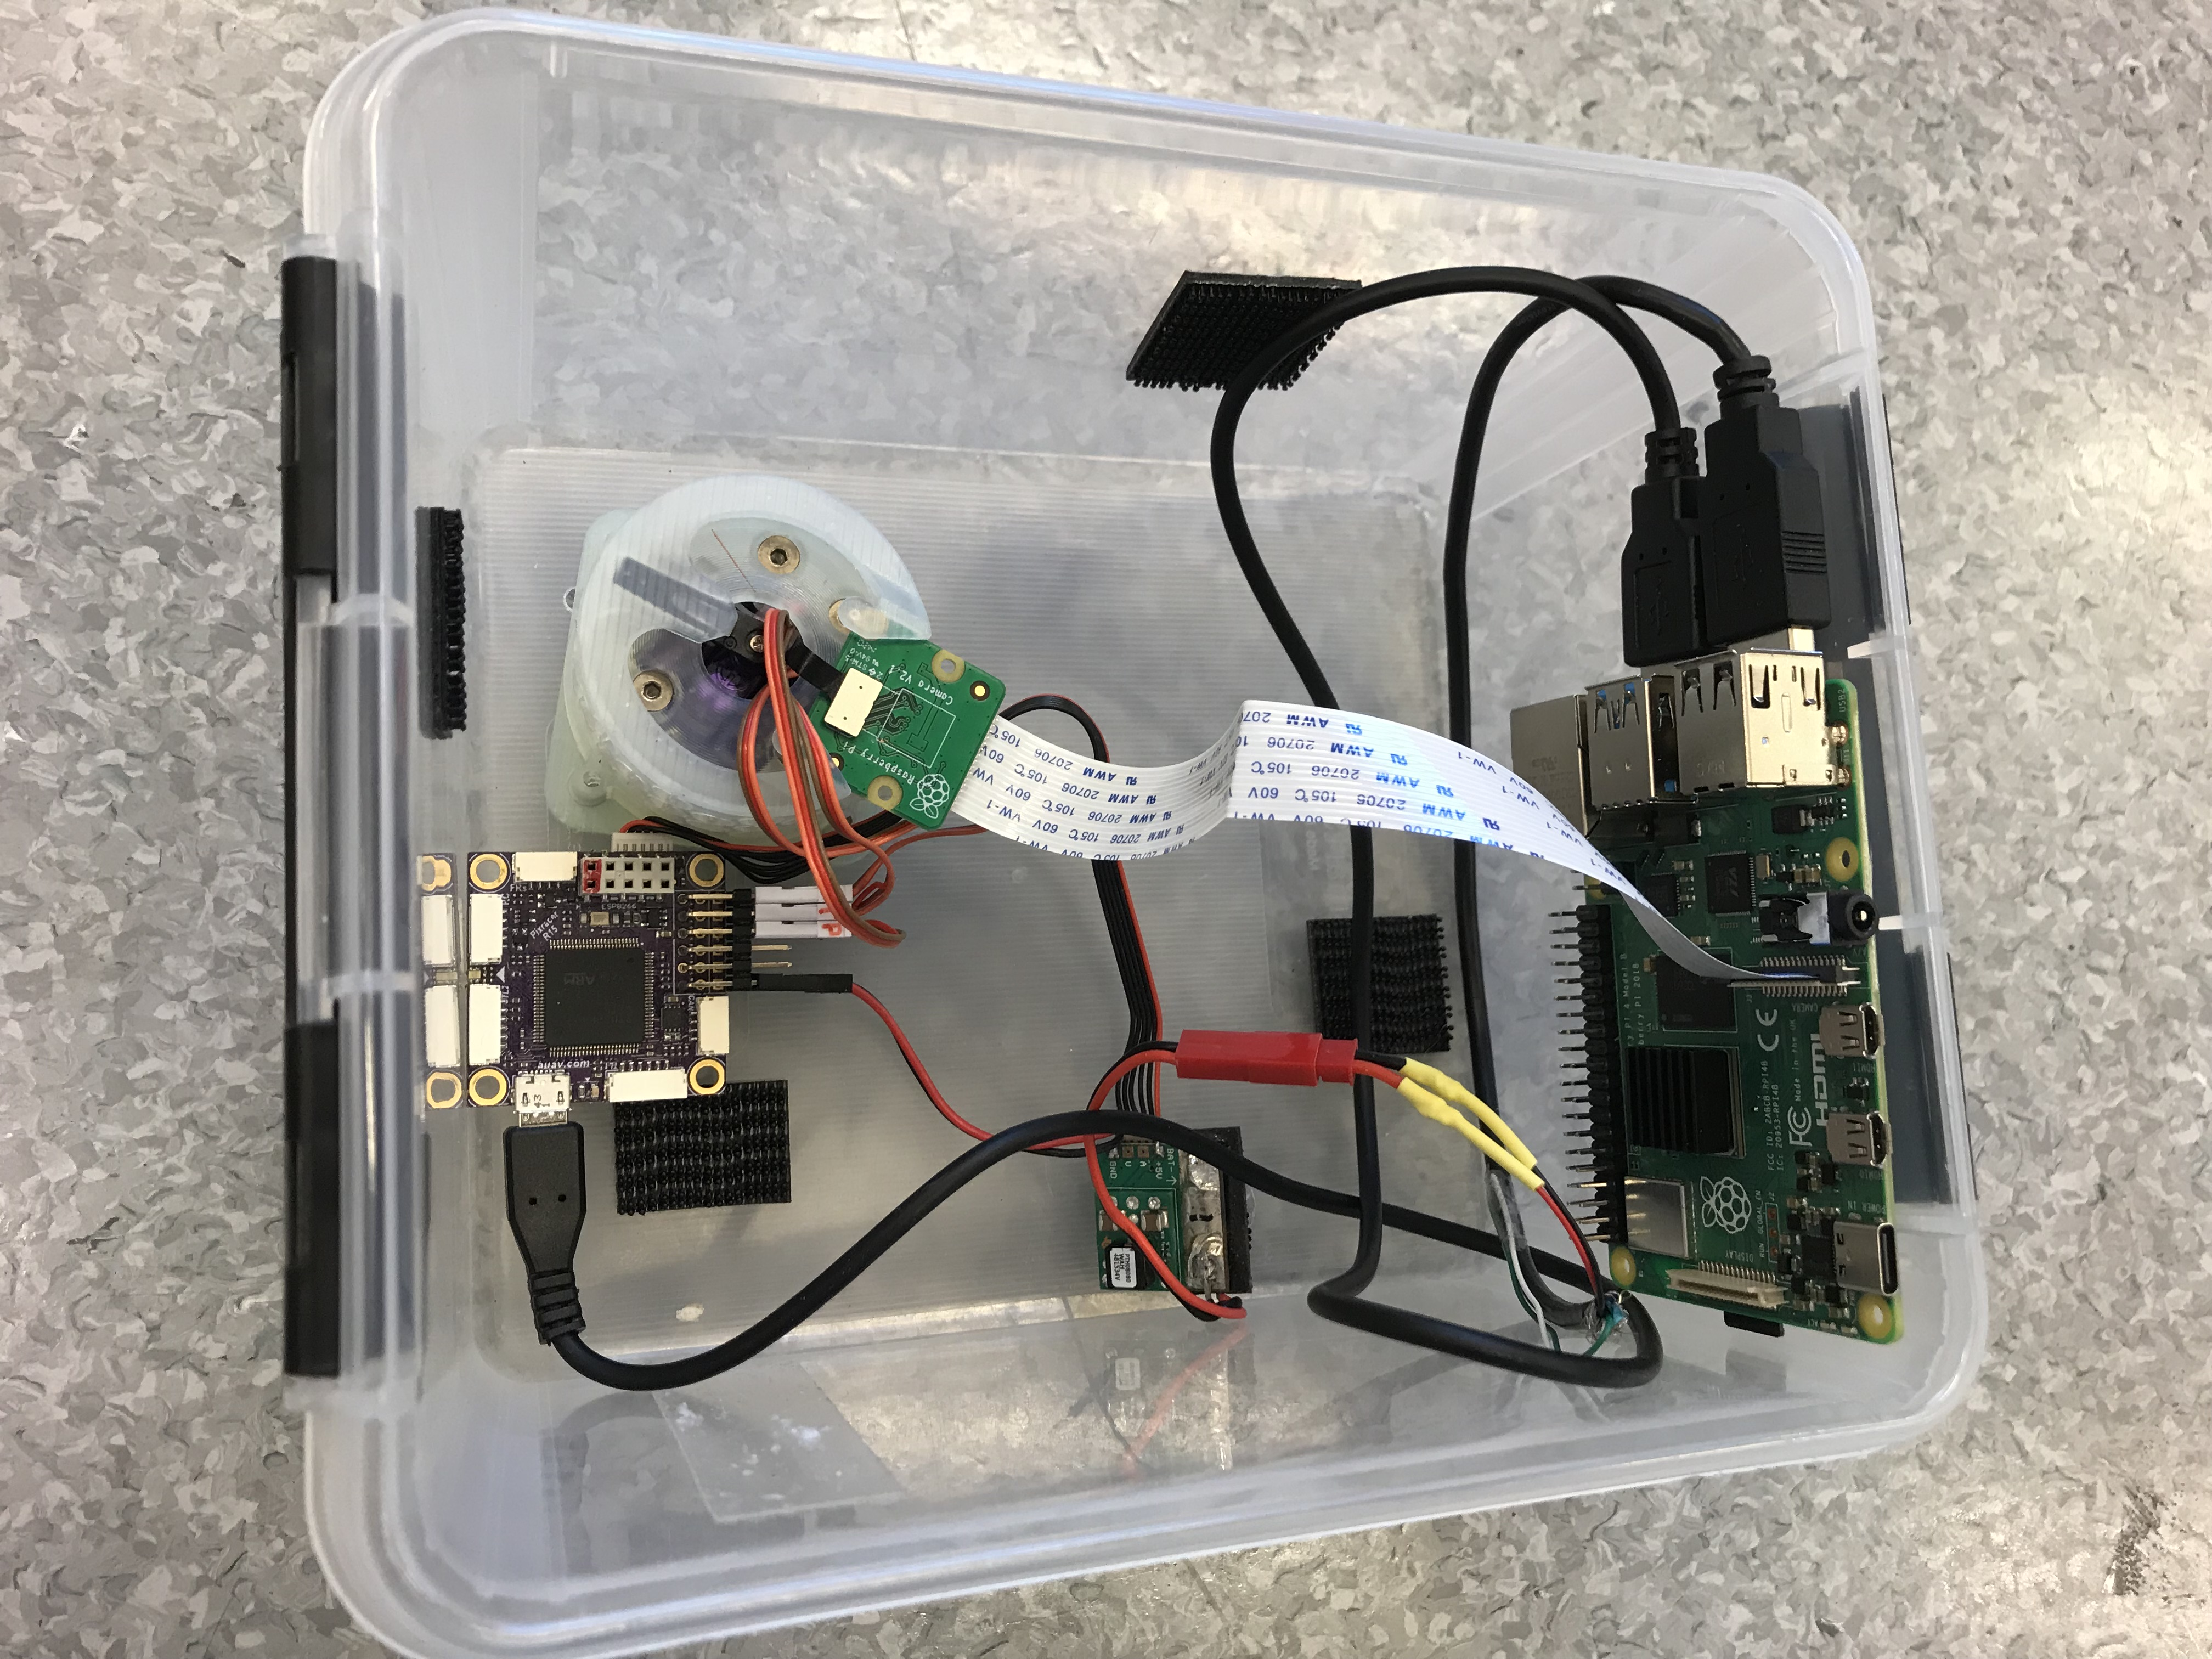
\includegraphics[width=.47\textwidth]{images/drone-box-1.jpg}\hfill
   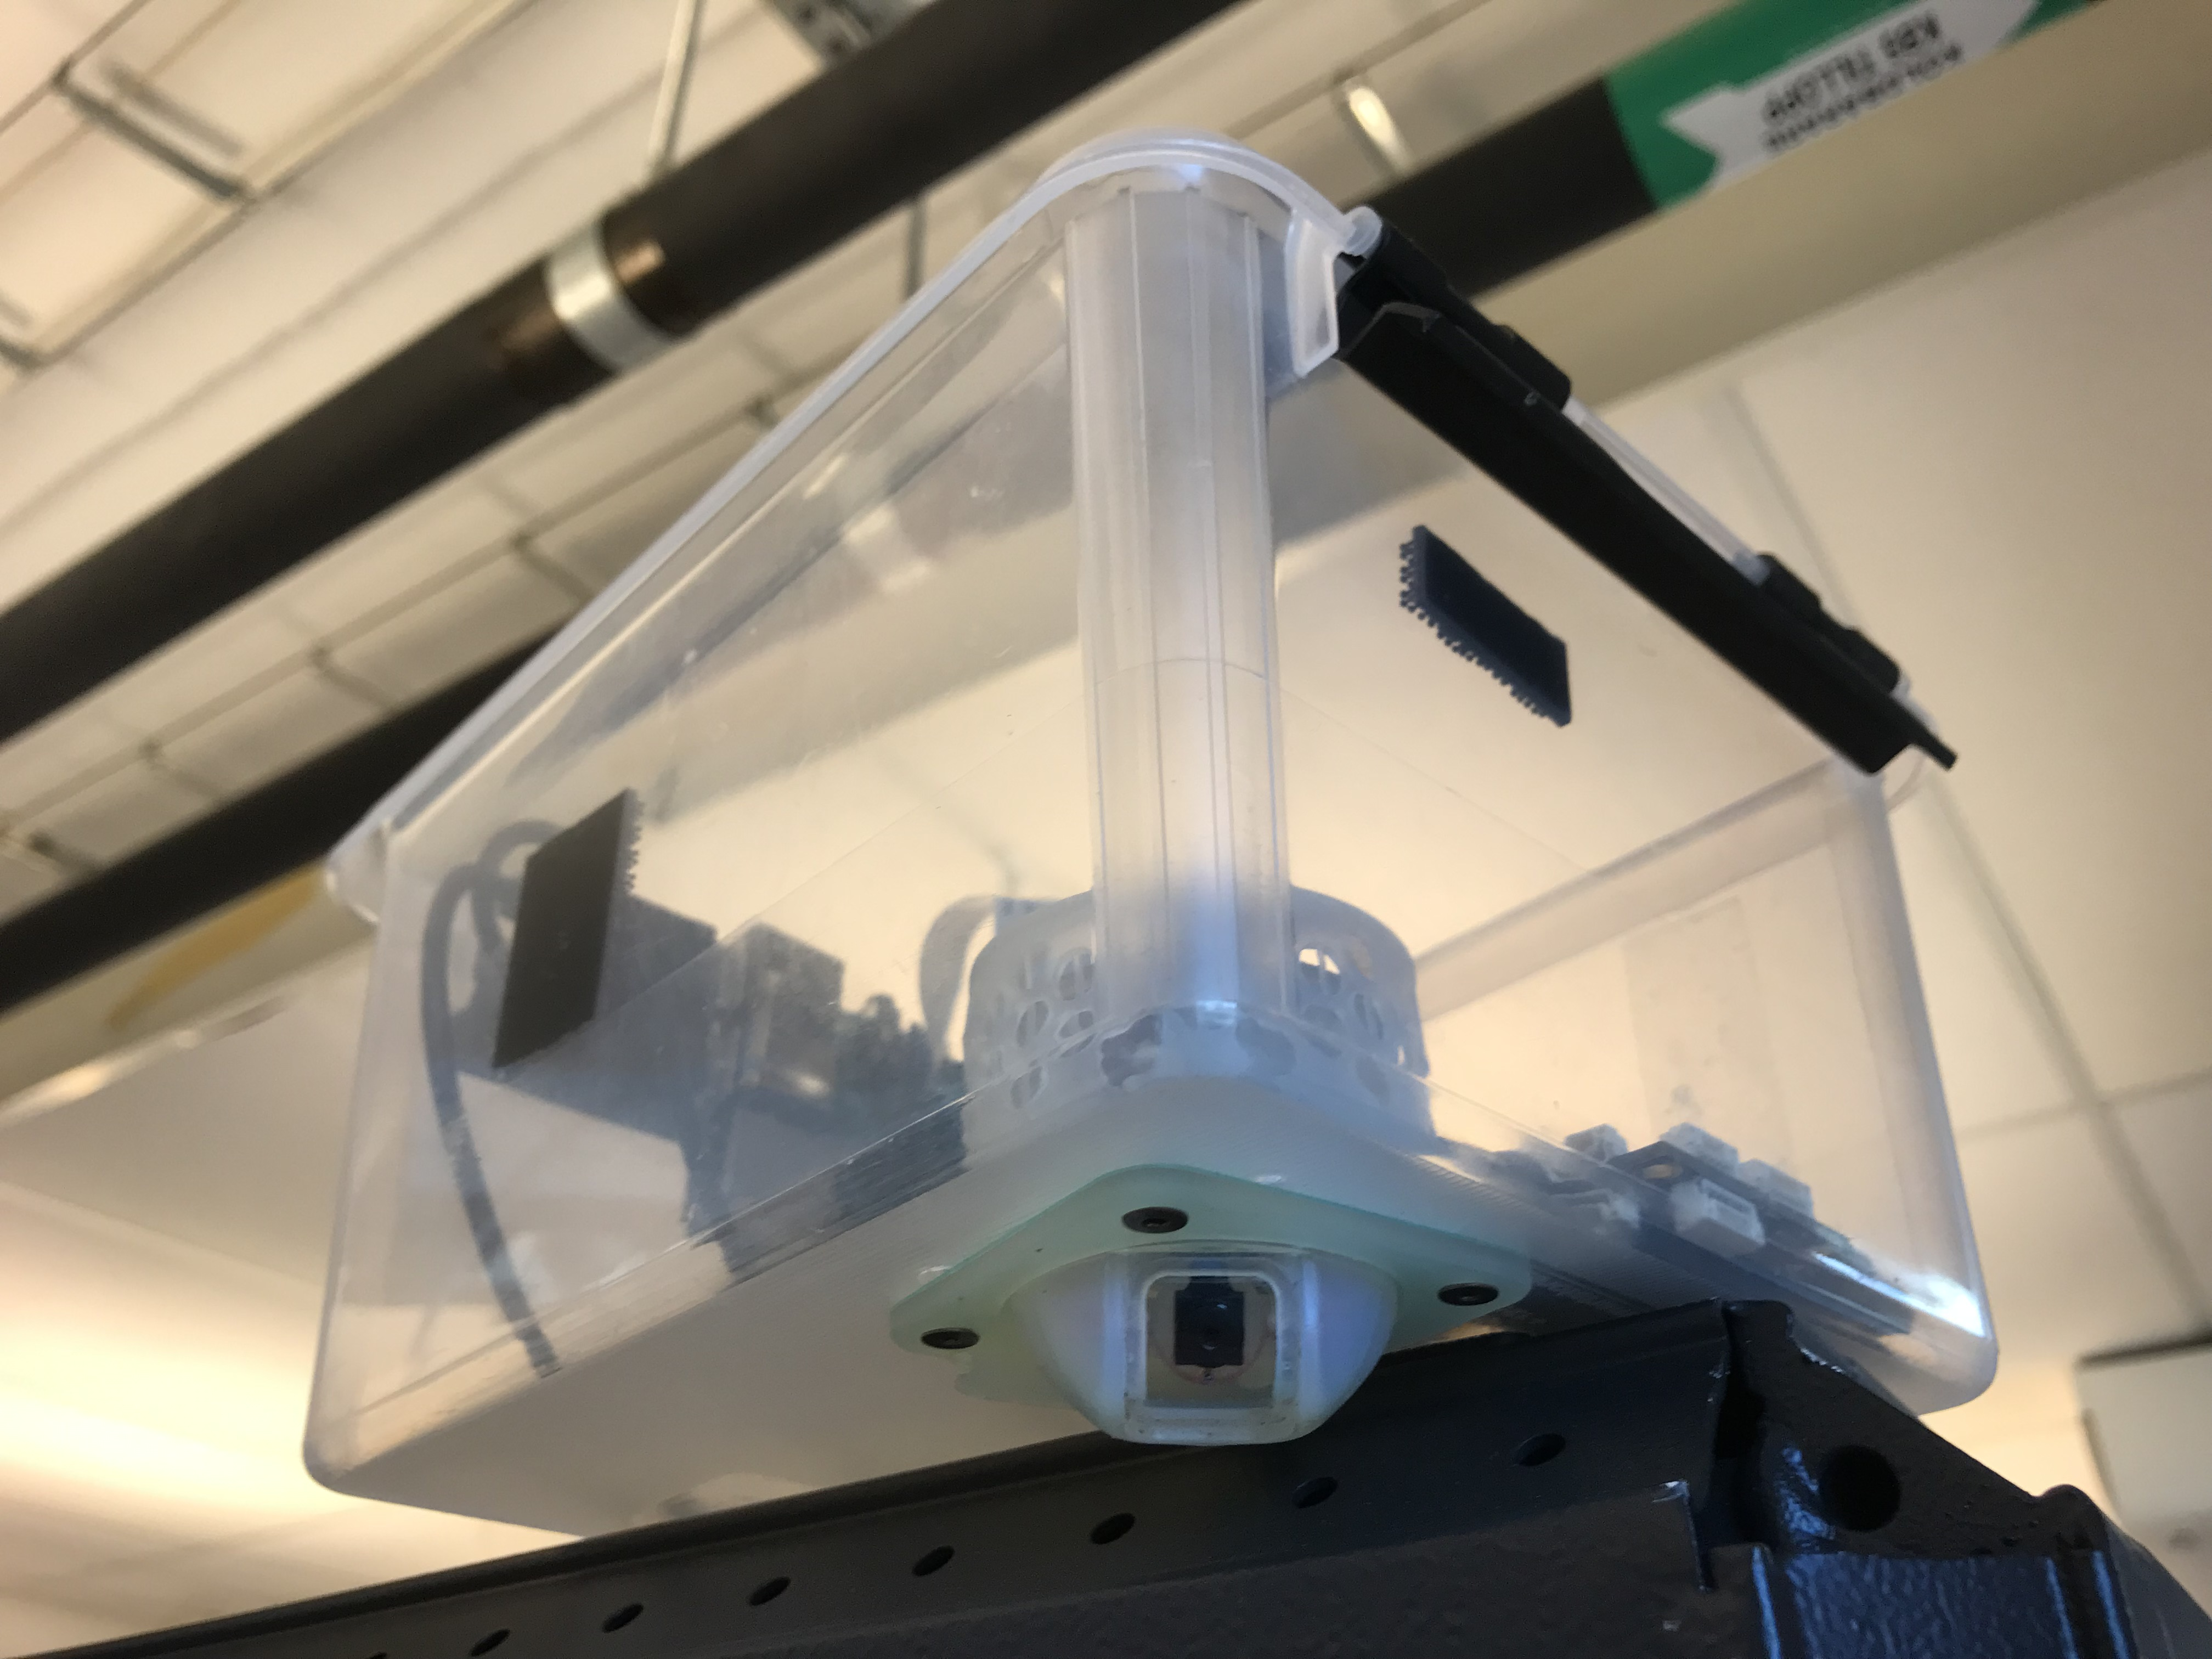
\includegraphics[width=.47\textwidth]{images/drone-box-2.jpg}
   \caption{The box that houses the drone hardware for the experiment. The left picture shows the box from above, from the left the following components are visible: flight controller, gimbal with camera module, power supply and Raspberry Pi. The right image shows the box from the outside.}
   \label{fig:drone-setup}
\end{figure}

\section{Software}
This section will go through the finished components of software that were used in the test bed.

\begin{description}
   \item[Firmware: ArduPlane]
   The firmware running on the flight controller is called ArduPlane, which is part of the open-source autopilot software suite ArduPilot that enables the creation of unmanned, autonomous vehicles \cite{ardupilot-org}. It is developed by a community of developers and is available on GitHub \cite{ardupilot-github}.
   
   \item[Protocol: MAVLink]
   As can be read on their website \cite{mavlink}, MAVLink is a lightweight protocol suited for communication with drones and between drone components. It has a byte overhead of 14 bytes and allows for concurrent communication between up to 255 systems. 
   
   \item[Package: pymavlink]
   This package is a Python interface to communicate with MAVLink devices, available at \cite{pymavlink}. In the test bed software it is used to send control-commands to the drone.

   \item [Software: MAVProxy]
   MAVProxy \cite{mavproxy} is a software running on the companion computer whose task is to relay MAVLink messages from the control station to the flight controller. In the test bed it relays messages between the ethernet port (application) and the serial port (drone box). 

   \item[UV4L]
   UV4L is a video streaming server that supports real-time communication protocols and video encodings \cite{uv4l}. It's function in the test bed is to stream the local video feed to the web. 
   
   \item[Janus Server]
   As described on their webpage \cite{janus}, Janus is a plugin-based software that helps establish WebRTC connections. In this thesis it is used to establish the connection between the UV4L server and the web browser, enabling the peer-to-peer connection between the two devices.
\end{description}

\section{Gimbal Control Interface}
Using the software components previously named, a program serving as the gimbal interface for the operator was implemented in Python. The software takes joystick inputs from a PlayStation-controller and sends messages updating the position of the gimbal with desired delay, while also displaying the video feed in a window. The same software was also modified so that it could record the video being displayed to the operator. A visual overview of the system is shown in Figure \ref{fig:system-overview}.
\begin{figure}[!hbt]
   \centering
   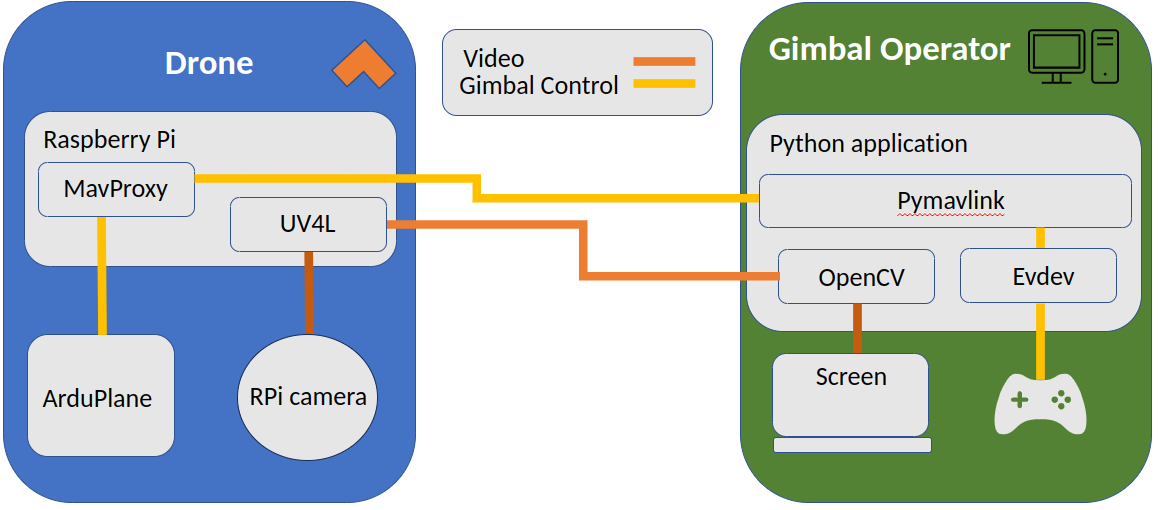
\includegraphics[scale=0.5]{images/system-overview.png} 
   \caption{An overview of the entire system. On the left, the drone and it's components including the RPi, RPi camera module and the flight controller are shown. On the right, the ground station and its' components including the web application, Janus server and the controller are shown. The colour of the connections represent what data they transfer, where orange is video, orange double-line is video negotiation and yellow is control.}
   \label{fig:system-overview}
\end{figure}

\section{Result Script}
In order to get results from the recorded video of each subject a script was implemented that was run on each trial, measuring the error of the operator in each video frame and saving it to a file.

\section{Hoverboard robot}
To make the object that was to be followed move, a hoverboard from another project was used. The hoverboard has four wheels and can be controlled by a game controller or follow a set of points using coordinates for which it uses a Lidar and SLAM-algorithm. This makes it possible to have the hoverboard run in a programmed route with little error. The apriltag was fastened on top of the hoverboard as high as possible without blocking the lidar. A picture of the hoverboard with the apriltag mounted is shown in figure \ref{fig:hoverboard}.

\begin{figure}[!hbt]
   \centering
   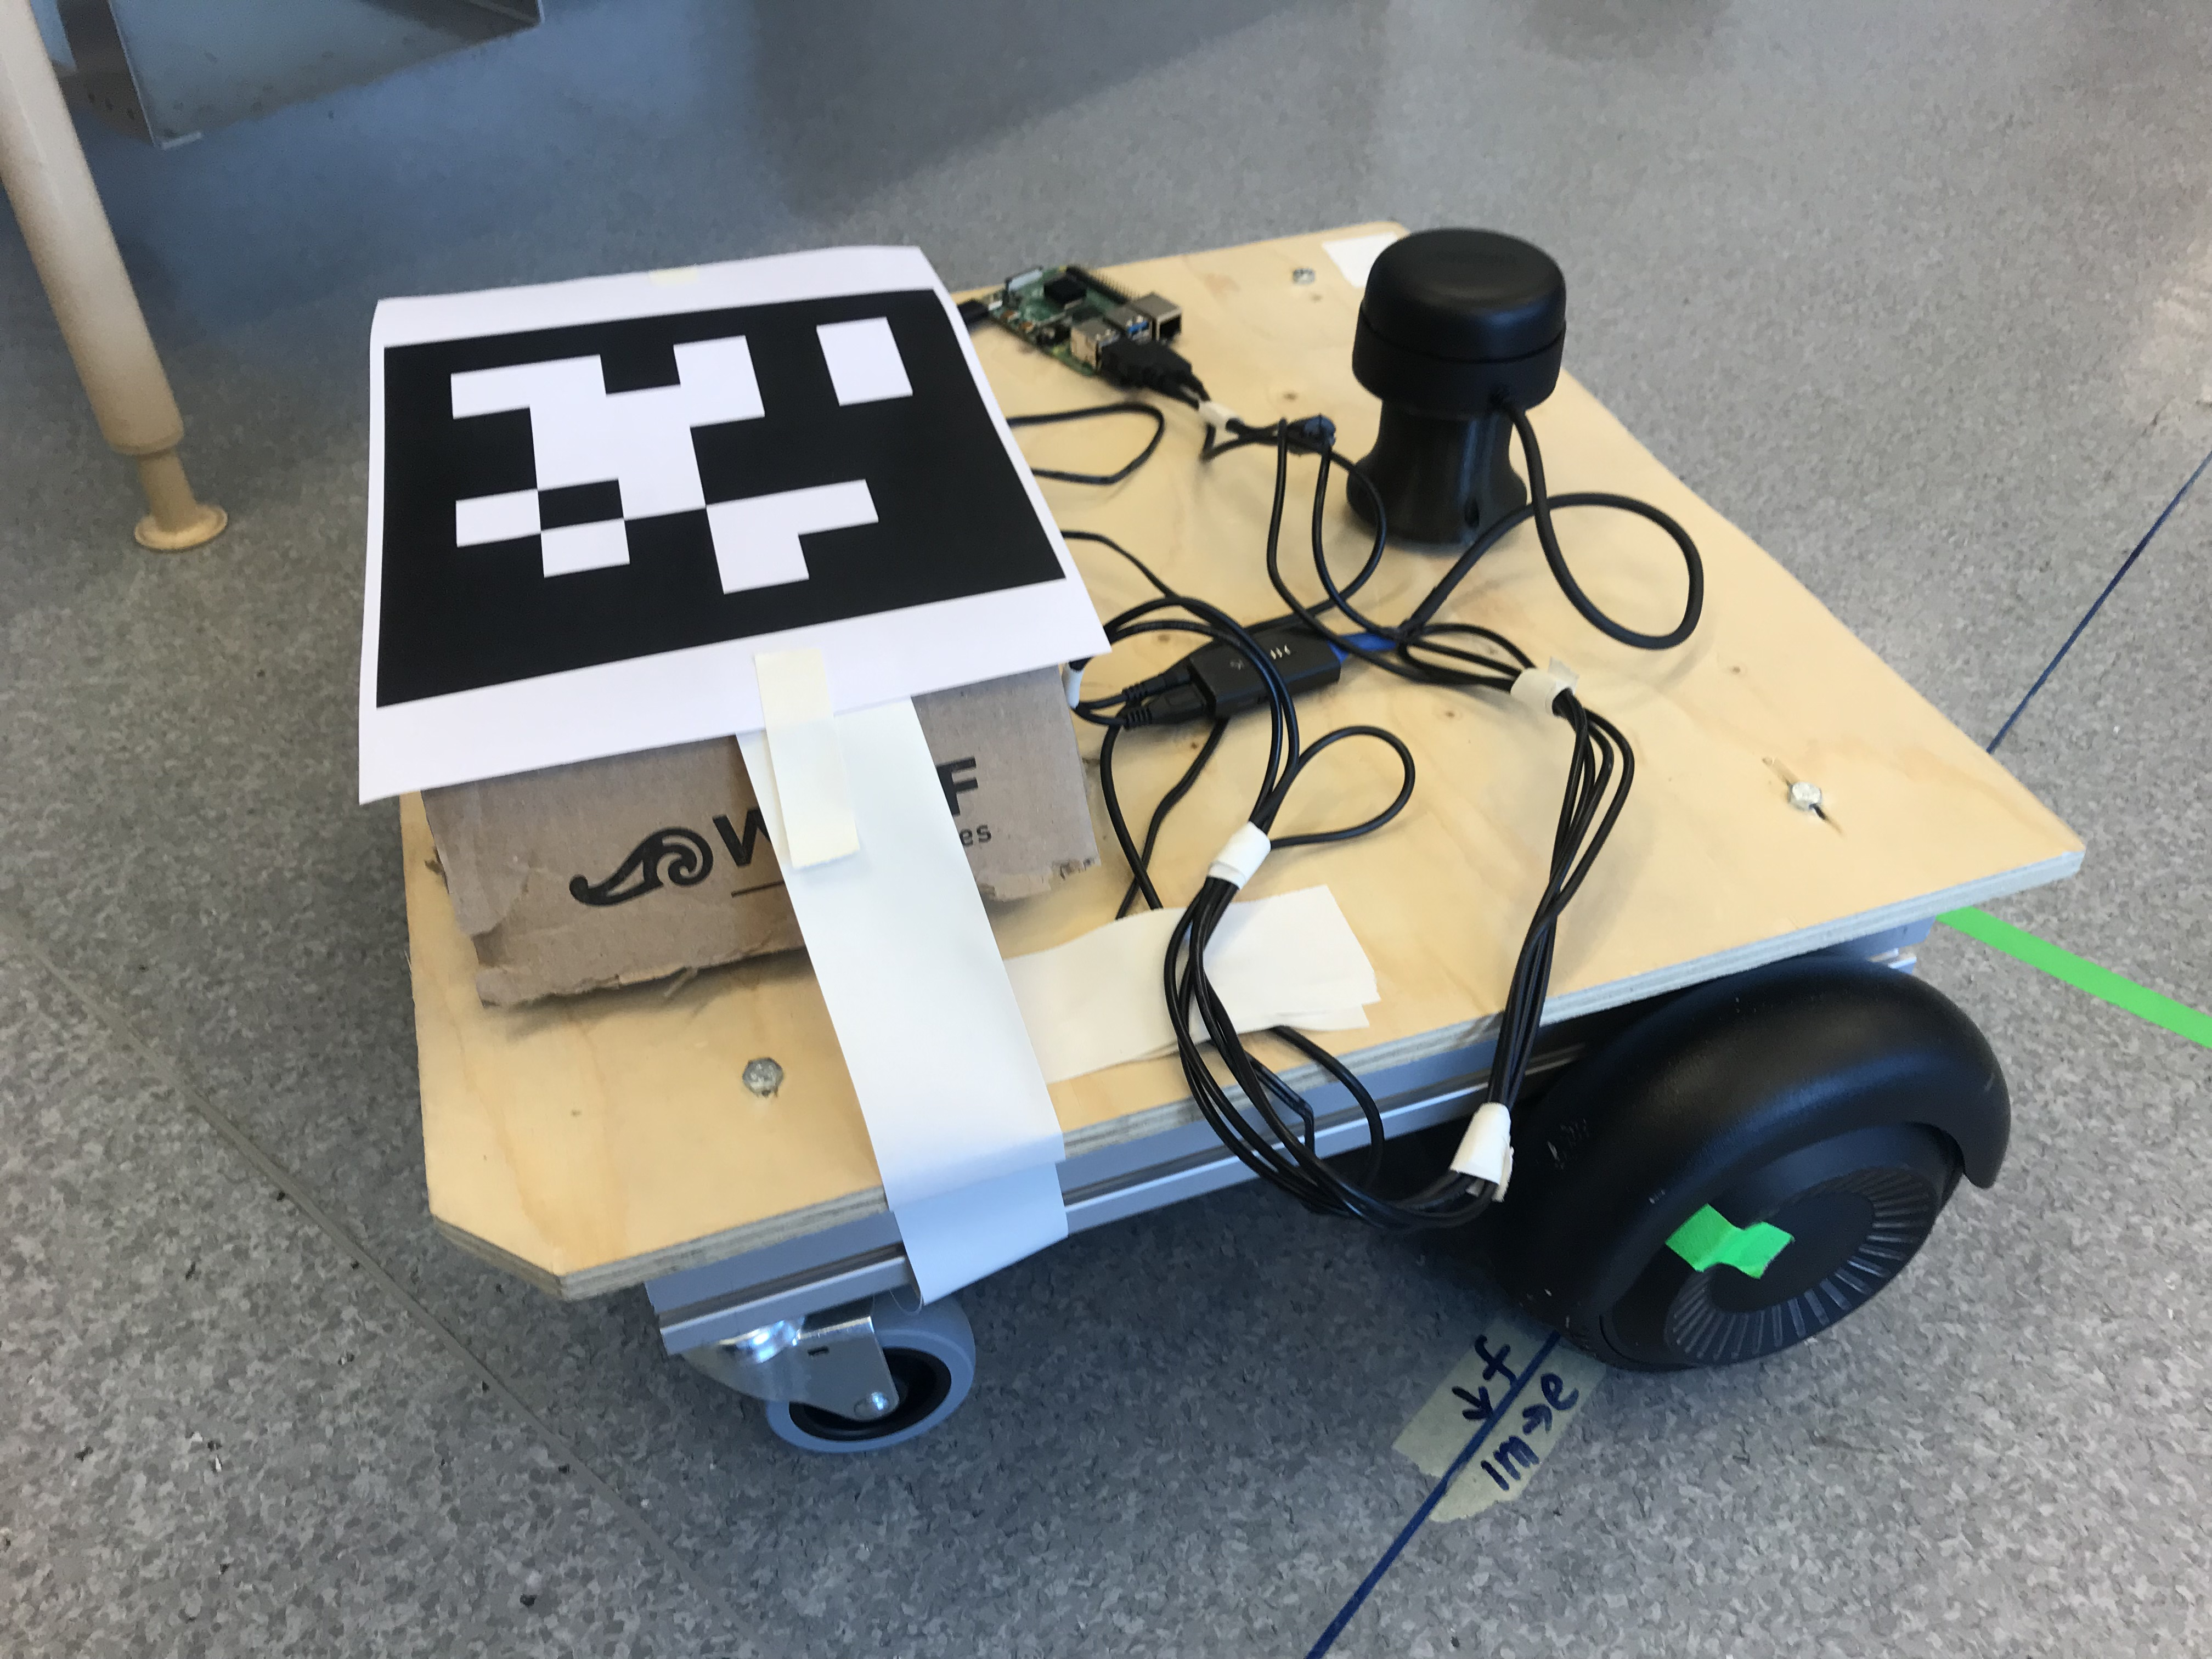
\includegraphics[scale=0.05]{images/hoverboard.jpg} 
   \caption{}
   \label{fig:hoverboard}
\end{figure}

\chapter{Experiment}
This chapter will describe the experimental setup, procedure and evaluation.

\section{Experimental Setup}
The experiment was set up in a lab where the subject and the conductor sits at a desk with a high shelf behind them obscuring the view towards the rest of the lab. Behind the shelf the robots used in the experiment are located. An illustration of the lab setup is provided in figure \ref{fig:exp-setup}. 

\begin{figure}[!hbt]
   \centering
   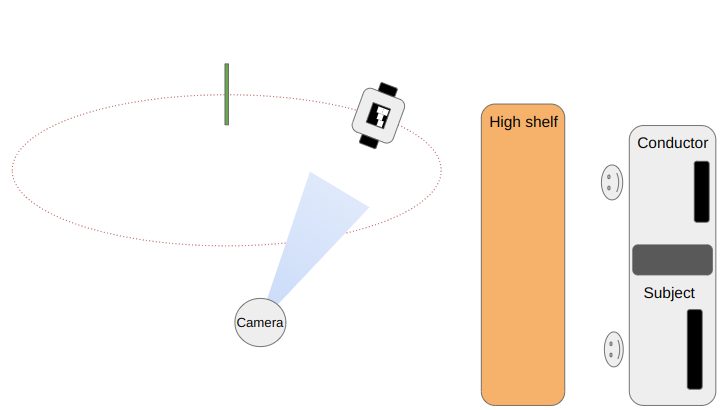
\includegraphics[scale=0.3]{images/exp-setup.png} 
   \caption{An overview of the experimental setup. To the right the experiment conductor and subject by a desk facing right. On the left side, behind the shelf, the test bed including the camera and the hoverboard are located. The camera is mounted at a height of 2.1 meters with the gimbal facing down.}
   \label{fig:exp-setup}
\end{figure}

An image of the hoverboard and the camera is shown in image \ref{fig:real-exp}.

\begin{figure}[!hbt]
   \centering
   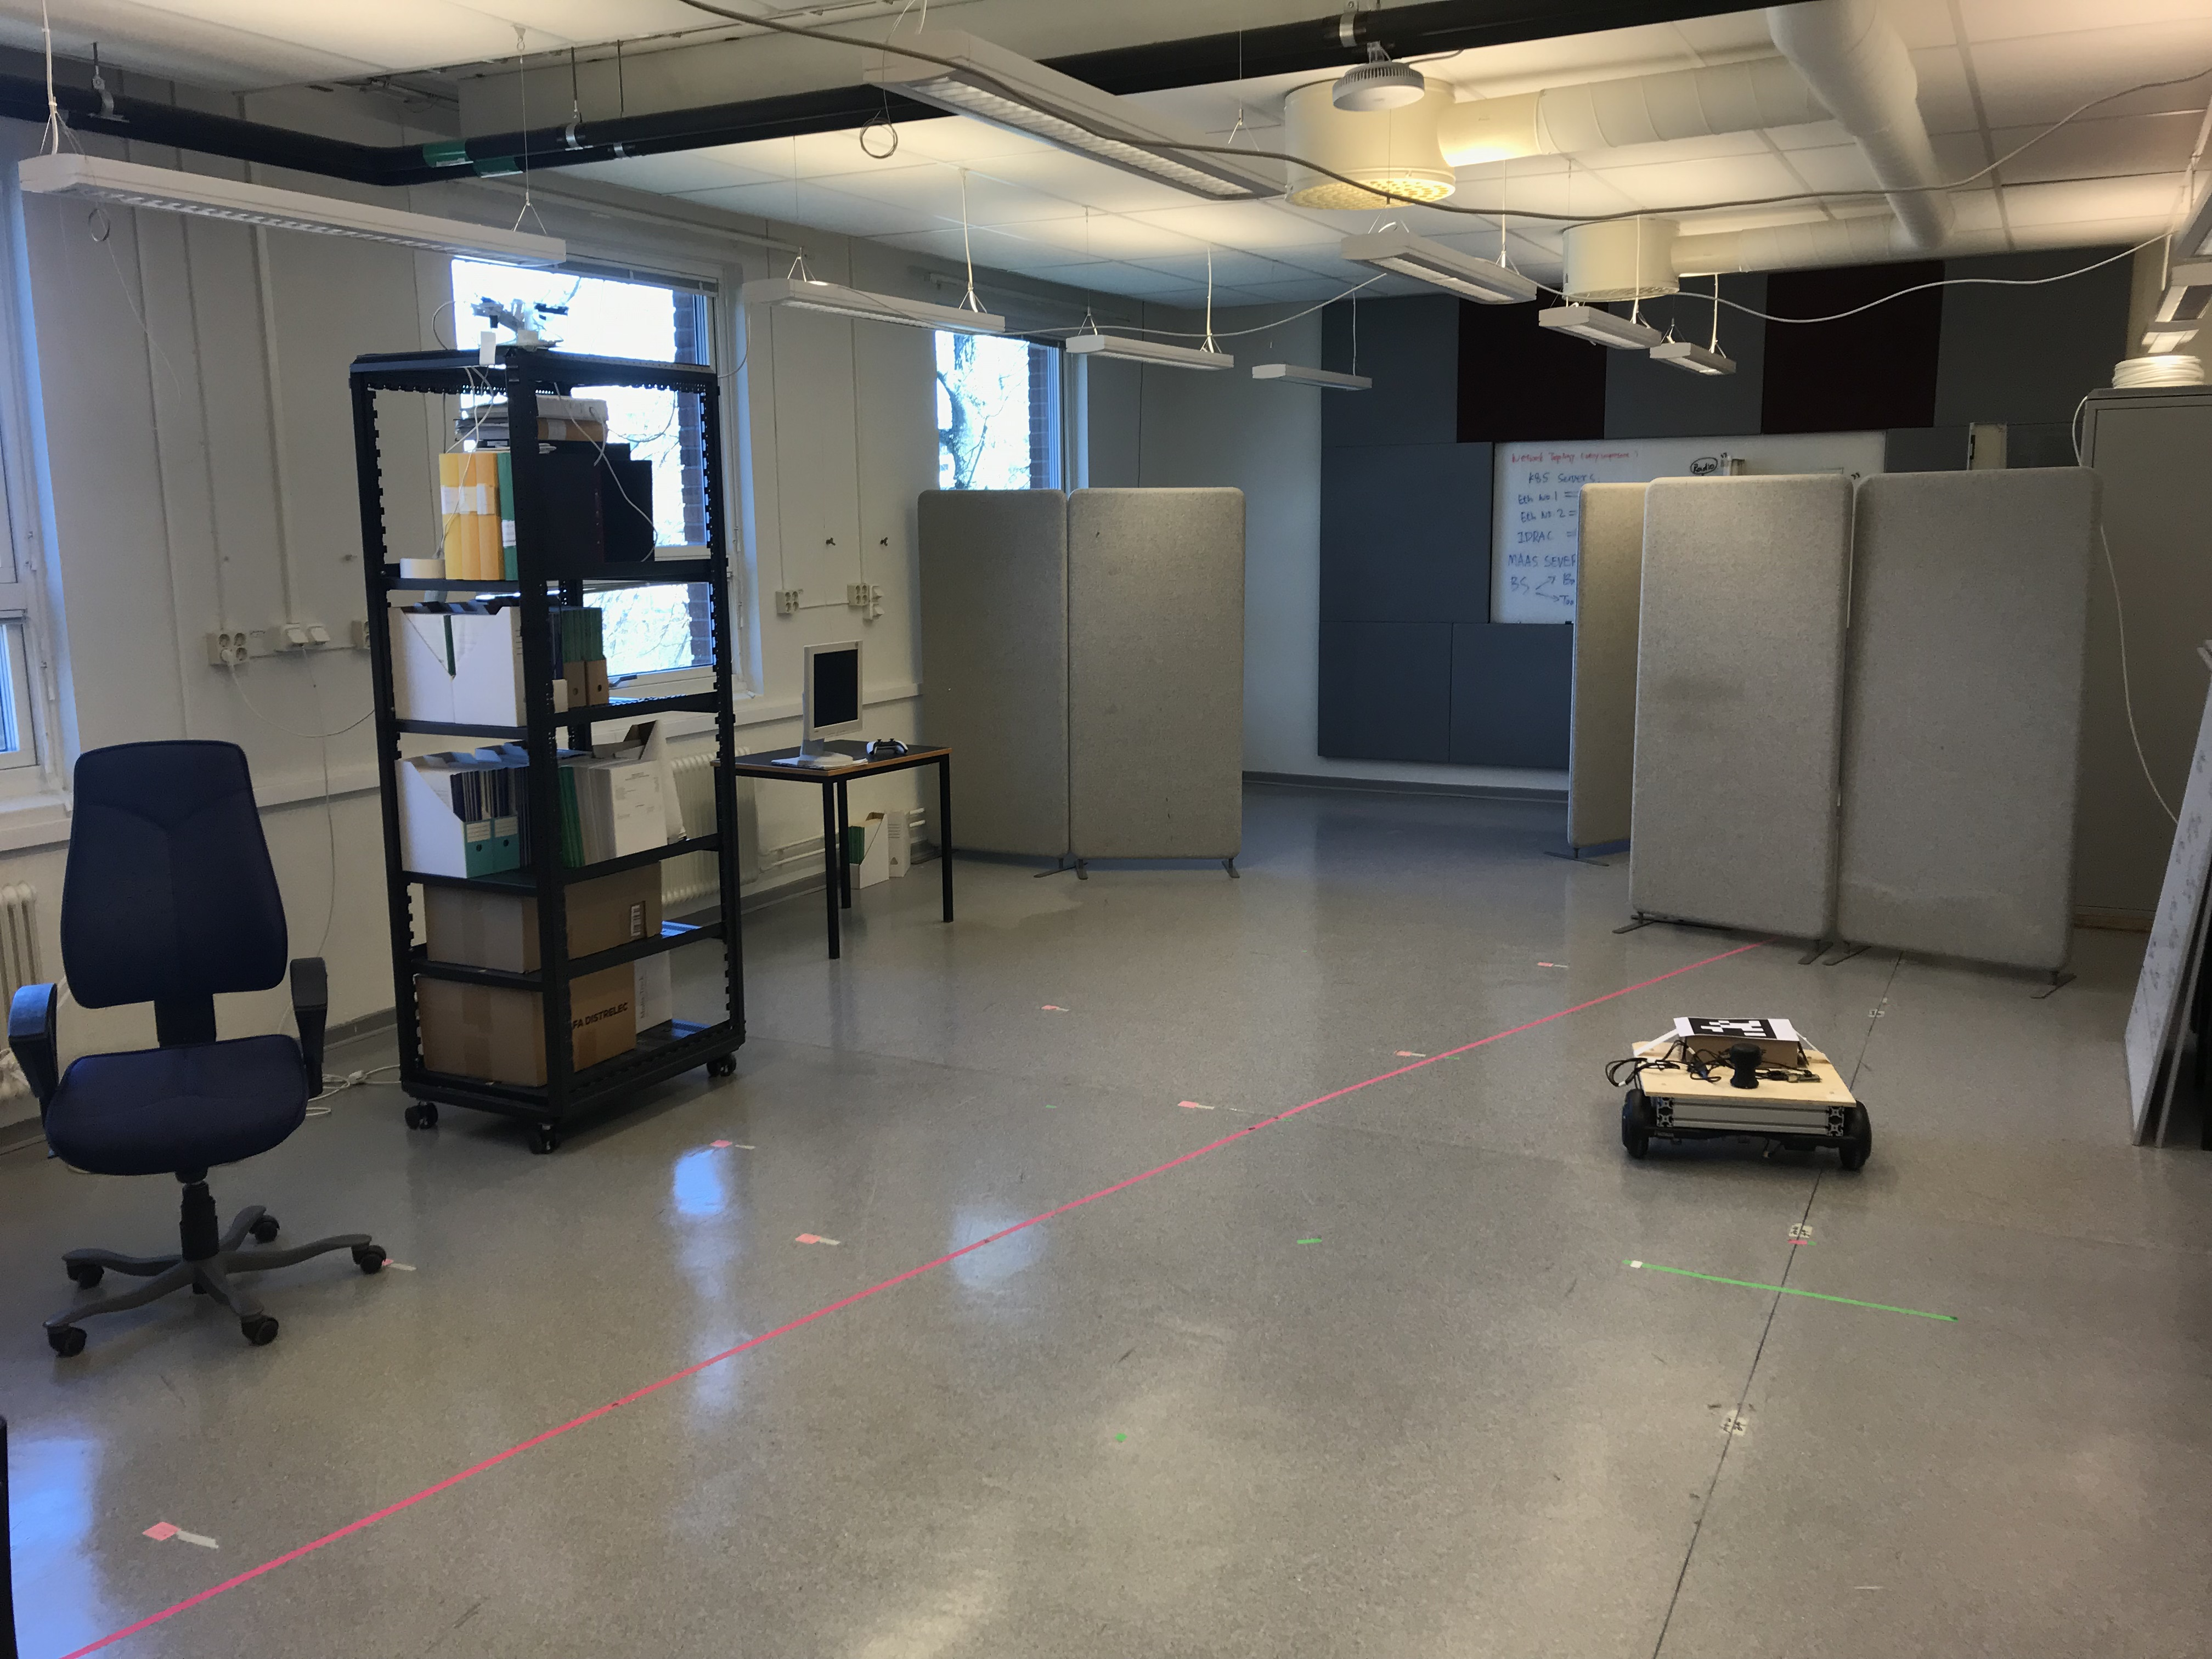
\includegraphics[scale=0.1]{images/testbed.jpg} 
   \caption{A picture of the test bed. On the left side there is a server rack with the drone box mounted on top. The hoverboard can be seen on the right side of the picture.}
   \label{fig:real-exp}
\end{figure}

\subsection{Subject selection and recruitment}
The subjects were recruited mostly from the conductor's network of contacts, as in order for the subjects to be covered by insurance during the experiment, the subjects had to be either be students or employed by Lund University. Some of the participants came spontaneously while others booked a time in a spreadsheet provided by the conductor.

There were 10 test subjects, 4 women and 6 men, with an average age of 26.1 years where the youngest was 23 and the oldest 37. Furthermore, they were questioned about their eyesight, handedness as well as experience with FPV-games and flying drones.

There was no compensation for the subjects other than home baked goods and a hot beverage, which were offered at the beginning of each experiment. 

\subsection{Lab Conditions}
The lab is located in the E-building at LTH, Lund University. It can also be mentioned that the windows in the room face north, so there was no risk of direct sunlight during the experiments.

\section{Experimental Procedure}
In this section each of the steps will be described in more detail. The experimental procedure is summarized in the table \ref{tab:task-timeline}.

\begin{table}[ht]
   \centering
   \caption{Task Timeline}
   \label{tab:task-timeline}
   \begin{tabular}{|c|l|l|}
   \hline
   \textbf{Time (approx.)} & \textbf{Task} & \textbf{Instruction} \\ \hline
   3 & Coffee and cookies & \\ \hline
   5 & Introduction & Tell the subject about what the study is about. \\
   & & Gather personal data + consent \\ \hline
   2 & SSQ & \\ \hline
   3 & Experiment walkthrough & What is going to happen \\
   & & Description of task \\
   & & Where to aim exactly on the apriltag \\ \hline
   2 & Warm-up & The subject gets to try the setup for one lap \\ \hline
   10 & Tests & 5 tests with added latencies [0, 200, 300, 400, 500] \\ 
   & & in random order \\ \hline
   2 & SSQ & \\ \hline
   3 & Interview & \\ \hline
   30 & Total & \\ \hline
   \end{tabular}
\end{table}

\subsection{Task}
The task was to keep the center of the screen, marked with a red dot, aligned with the center of the apriltag laying on top of the hoverboard (shown in \ref{fig:hoverboard}) while moving in an elipse.

\subsection{Introduction}
The experiment starts with the subject being seated at the desk to read through the consent form. After this was signed the conductor clarified that the subject was free to ask any question during the experiment and could choose to interrupt it without declaring any reason. 

Then, the subject fill out the background information form where they also get to choose a four digit code which from that point is the only identifier of the subject and it's results. If the subject booked a time slot in the spreadsheet, they were at this point removed from it.

\subsection{Task Description}
The interface was opened on the subject's screen and the task was explained. The subjects were also shown a printed apriltag with a cross on it, marking the spot where to aim on the tag. The particular apriltag printed for this experiment had two white and two black squares meeting in the middle, making the center easier to identify. The apriltag shown to the subject is shown in figure \ref{fig:apriltag}.

\begin{figure}[!hbt]
   \centering
   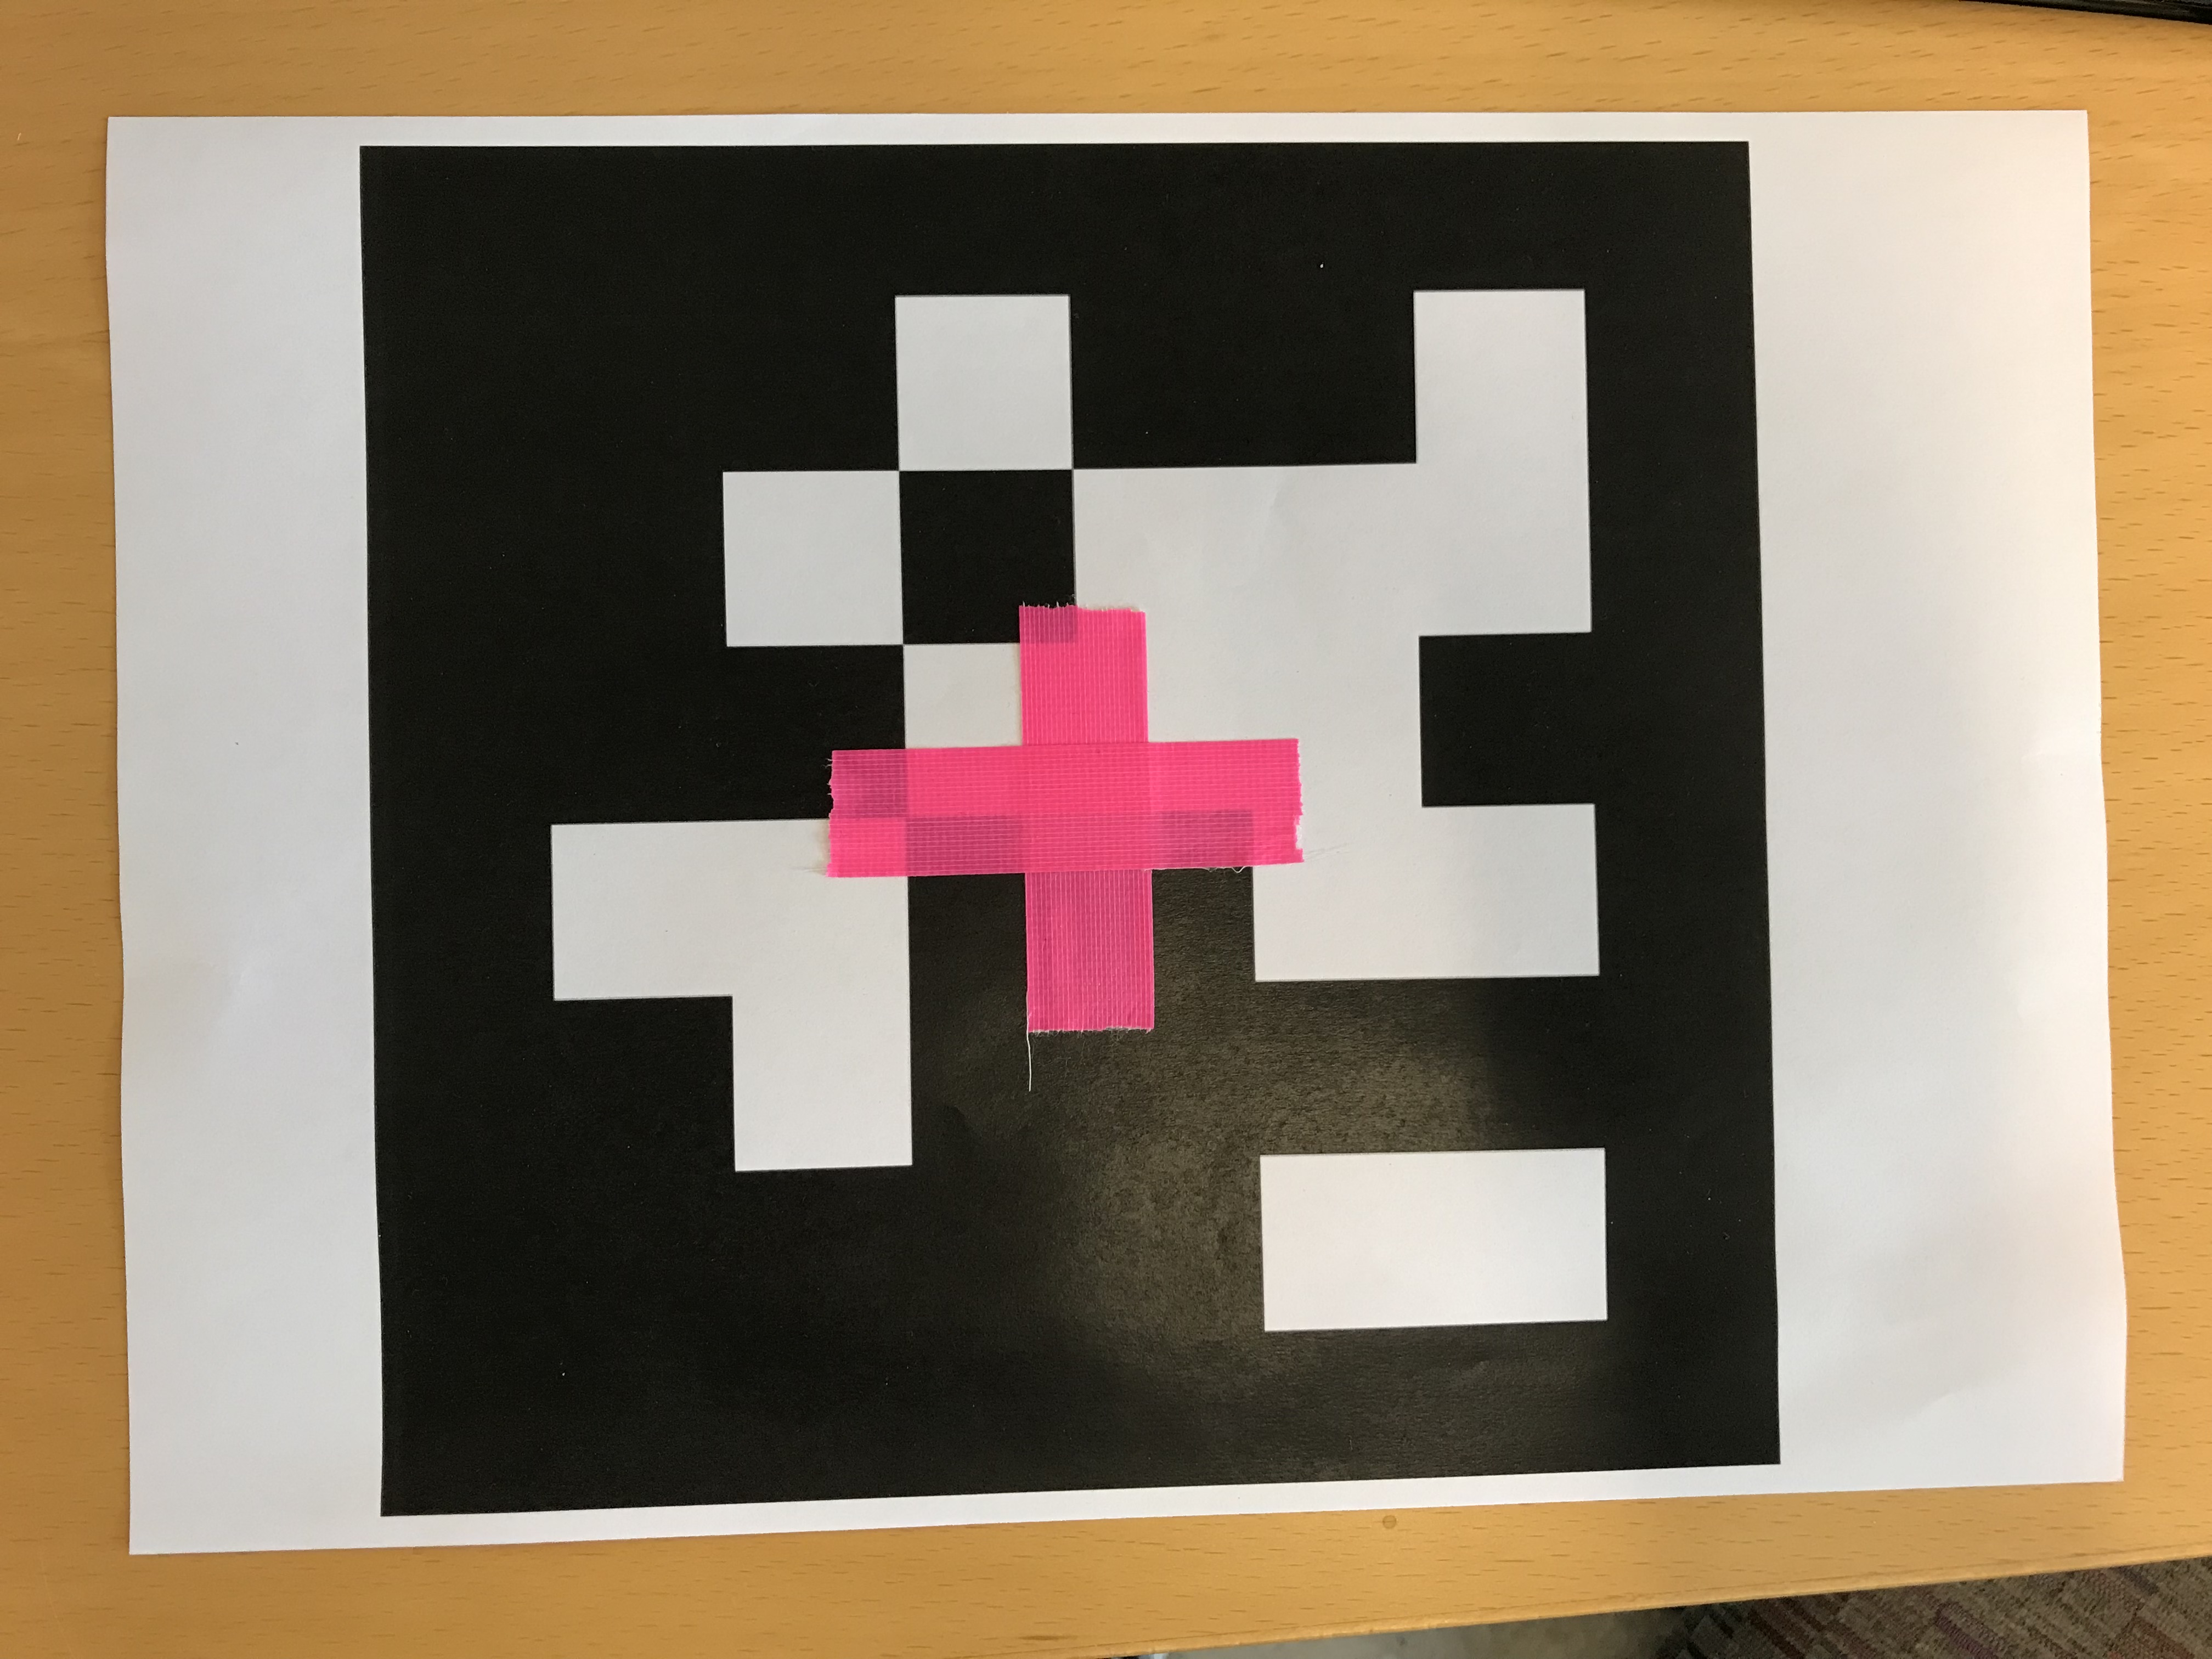
\includegraphics[scale=0.08]{images/apriltag.jpg} 
   \caption{The apriltag used to show the subject where to aim.}
   \label{fig:apriltag}
\end{figure}

The subject was then given a chance to try the system, and was given the controller and presented with the view. The hoverboard was started and ran for one lap in the same path that it would run during the test.

\subsection{Test Procedure}
After the task description and warm-up the tests commenced. The added latencies tested were 0, 200, 300, 400 and 600 and the order in which they were given to the subject was random. 
At the beginning of each trial the interface was restarted with one of the latencies induced in the system. The subject was then asked to put the red marker in the middle of the screen in the middle of the apriltag. When the subject confirmed that they were ready to start the conductor started the hoverboard. The subject followed the hoverboard for two laps, which took about 2 minutes in total.

After the laps were completed the interface was shut down and the subject was asked to rate the system by answering four different questions on a scale from 1 to 5. When the subject had answered the questions the next trial was started.

At the end of the fifth and last trial the subject got to fill in the sickness questionnaire was also asked a few interview questions by the conductor.

\section{Evaluation}
The following two sections will describe the quantative and qualitative methods that are used to evaluate the performance of the system.

\subsection{Quantative Evaluation}
To measure each subjects performance, each trial was recorded and a script using a detection algorithm gave the distance between the red dot and the center of the apriltag.    

\subsection{Qualitative Evaluation}
After each trial the subject answered a form with four questions about the system on a scale from 1-5, labeled 'terrible' to 'excellent'. The questions were the following:
\begin{enumerate}
   \item How would you describe the controllability of the system?
   \item How would you rate your ability to perform the task?
   \item How would you rate your experience of the system?
   \item How would you rate your impression of the system as a whole?
\end{enumerate}

Right after the last trial the subject filled out the SSQ once more. Then, a brief interview was conducted with the following four questions:
\begin{enumerate}
   \item What was your general experience of controlling the camera?
   \item Did you experience any difference in the controls between the trials?
   \item Was there any part of the track that was harder than any other?
   \item Do you think the system would have been usable with the worst experimental conditions?
\end{enumerate}

\subsection{Auto-follow mode}
As a proof of concept, an auto-follow mode was implemented in the application using real-time object detection of the video feed. Although it is not optimal to have that high latency introduced in the control-loop, it is of interest as the resource heavy object detection algorithm does not stress the hardware on the drone. The mode is evaluated with the same methods as the rest of the experiment, although the user is just passively watching the feed.

\section{Known Sources of Error}

\subsection{Frame detection accuracy}
The detection algorithm used to calculate the distance from the center of the apriltag to the center of the screen could sometimes during fast camera movements not detect the apriltag. This resulted in a NaN value at that particular frame. The average percentage of frames detected where 85\%, with a minimum of 80\% and a maximum of 89\%. The percentage of frames detected was not found to be correlated with the delay and are plotted for each subject and delay in figure \ref{fig:frames-detected}. 

\begin{figure}[!hbt]
   \centering
   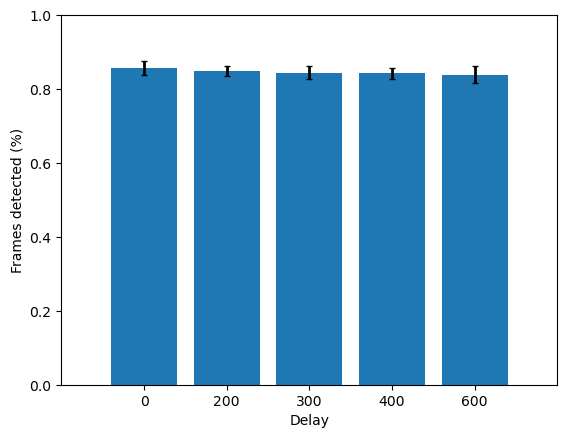
\includegraphics[scale=0.5]{images/frames-detected.png} 
   \caption{Form answers averaged for all subjects for each delay.}
   \label{fig:frames-detected}
\end{figure}

To make for better averages over different trials, all NaN values, i.e frames where no apriltag was detected in the frame, were linearly interpolated. To illustrate this one result is shown before and after interpolation in \ref{fig:raw-vs-interpolated}. 

\begin{figure}[!hbt]
   \centering
   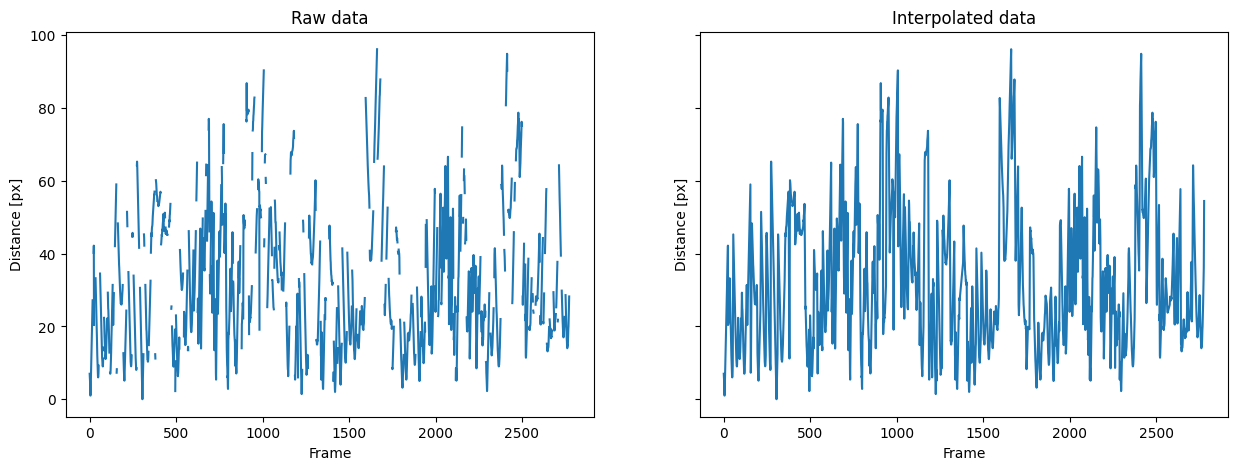
\includegraphics[scale=0.5]{images/raw-vs-interpolated.png} 
   \caption{Results for one trial: to the left the result with NaN-values and to the right interpolated result.}
   \label{fig:raw-vs-interpolated}
\end{figure}

\subsection{Difficulty of the task}
The center of the apriltag did not have a very clear center which could have made it difficult for the subject to complete the task. To remedy this a printed apriltag where the center was marked out, but it could be that the subject had difficulty identifying the exact center during the trial. 

\chapter{Results}
In \ref{tab:averages} the mean and standard deviation of the results are presented. The values are also visualized in plot \ref{fig:avg-std}.
\begin{table}[ht]
   \centering
   \begin{tabular}{|c|c|c|}
   \hline
   \textbf{Delay} & \textbf{ Mean} & \textbf{Std. deviation} \\
   \hline
   0 & 29.804138 & 18.030196 \\ \hline
   200 & 35.234192 & 22.347311 \\ \hline
   300 & 41.538190 & 26.805780 \\ \hline
   400 & 46.048449 & 28.718249 \\ \hline
   600 & 61.811312 & 37.226394 \\ \hline
   \end{tabular}
   \caption{Table caption goes here.}
   \label{tab:averages}
\end{table}

\begin{figure}[!hbt]
   \centering
   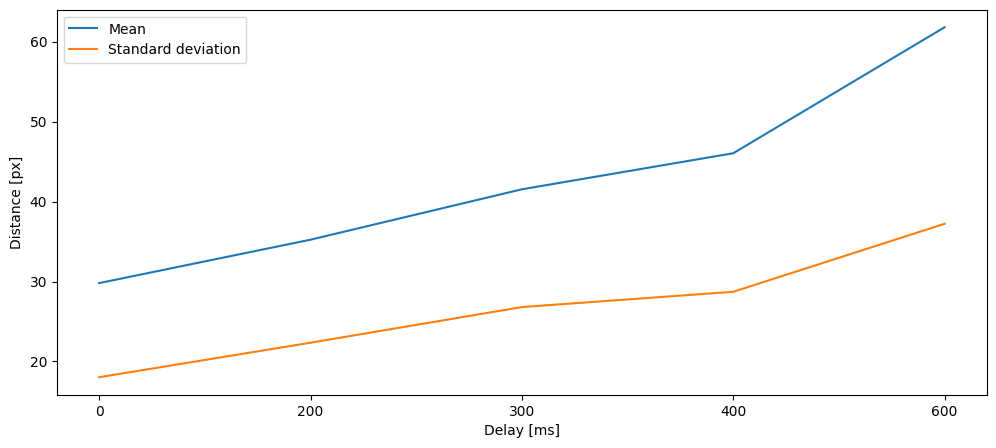
\includegraphics[scale=0.5]{images/avg-std.png} 
   \caption{Average and standard deviation for all delays.}
   \label{fig:avg-std}
\end{figure}

In figure \ref{fig:0vs600} the trials of all subjects have been summarized on a delay. The blue and green lines represent the summarized data while the orange and red lines represent a rolling average over 50 values. 

\begin{figure}[!hbt]
   \centering
   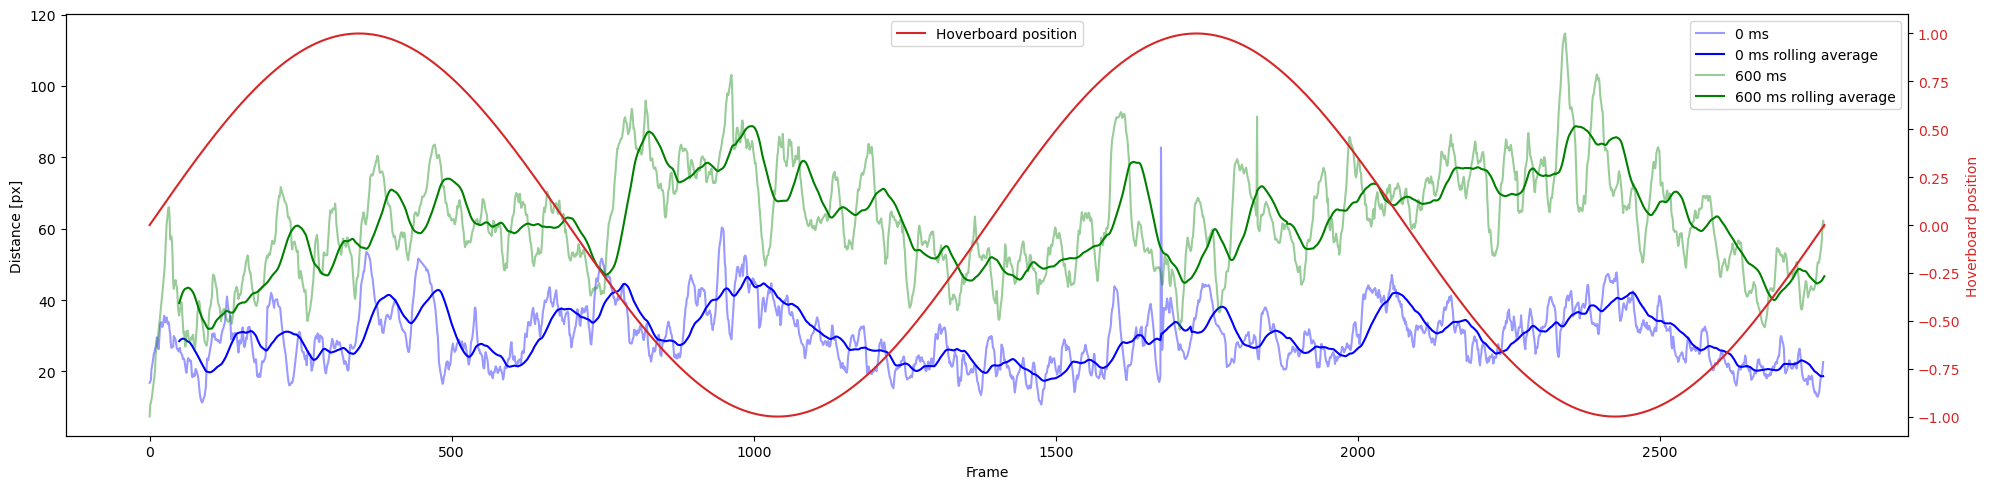
\includegraphics[scale=0.5]{images/0vs600.png} 
   \caption{Total trials for latencies 0 and 600 averaged over all subjects.}
   \label{fig:0vs600}
\end{figure}

In figure \ref{fig:ecdf} the ECDF over the averages at each delay is shown. The x-axis represents the value which the entry has while the y-axis represents the percentage of entries that are less than or equal to the x-axis value.

\begin{figure}[!hbt]
   \centering
   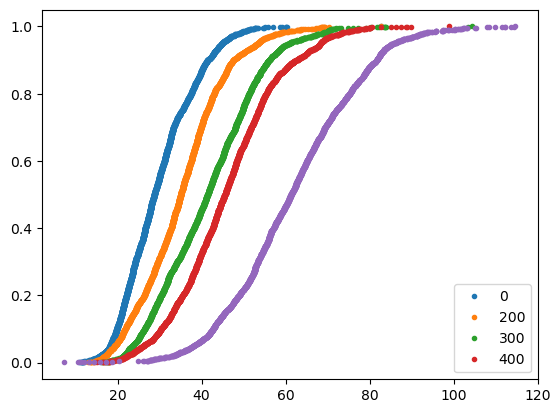
\includegraphics[scale=0.5]{images/ecdf.png} 
   \caption{ECDF of the total distance for all subjects.}
   \label{fig:ecdf}
\end{figure}

\begin{figure}[!hbt]
   \centering
   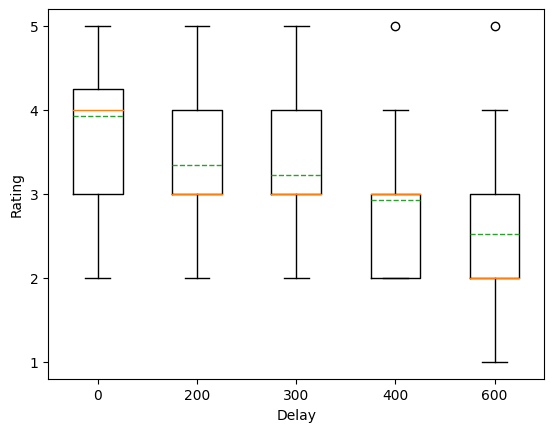
\includegraphics[scale=0.5]{images/form-ans.png} 
   \caption{Form answers averaged for all subjects for each delay.}
   \label{fig:ecdf}
\end{figure}

In figure \ref{fig:hoverboard-pos} all the values from the trials have been averaged and the position of the hoverboard has been superimposed.

\begin{figure}[!hbt]
   \centering
   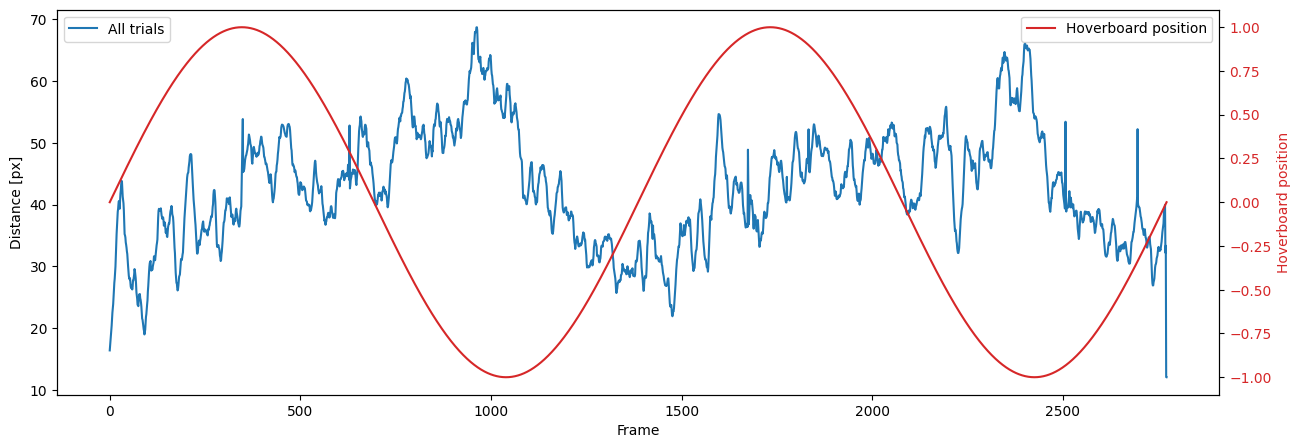
\includegraphics[scale=0.4]{images/hoverboard-pos.png} 
   \caption{All trials averaged with hoverboard position superimposed.}
   \label{fig:hoverboard-pos}
\end{figure}

\chapter{Discussion}
\section{Sources of error}
\subsection{Frame detection accuracy and interpolation} 


\section{System Architecture (SKRIVA DET SOM QOS?)}
Although being a bit outside the research scope of the project, a natural consequence has been to evaluate the strengths and weaknesses of different system architectures that could be implemented for real drone missions. This section will bring up some of the requierments from SSRS along with the particular architectures considered for the application of sea rescue.

\subsection{Main goals}
Being a real-time application over the Internet, there are many parts of the system that can introduce latency and efforts to reduce it can be boiled down to two actions: 
\begin{itemize}
   \item reducing the amount of processing agents between the operator and what is being controlled
   \item reducing the amount of processing time at the processing agents
\end{itemize} 
However, while one particular architecture might meet requierments in one area, for example latency, it can make other parts of the system more complex or computationally expensive. The task is inherently complex as there are many tradeoffs that have to be balanced and the requierments of the particular application has to be very clear. Difficulty of implementation as well as extendability are also important factors to consider. 

\subsection{WebRTC and data channels}
The use of WebRTC along with Janus enables two units to talk to one another directly over the web, removing a potential server that has to process the video feed and the relay it forward. However, if one would like to record the video and save it on a server the feed now has to be redirected to the server from either the system of the end user or the drone itself. 

One part of WebRTC that was of particular interest during the implementation was data channels. These are meant to be utilized to send small amounts of data along with the videopackets utilizing the already established P2P to transmit for example a time stamp or control commands. In UV4L it is possible to check a box that automatically ties the gyroscope of a device to the output of three servos. Since the control in this project goes through the Ardupilot firmware one would need to implement a relay running on the companion computer, which there was not time for in the implementation part of this project. 

\chapter{Conclusion}

\chapter{Future Work}


% Should use consistent formatting when it comes to Names ("FirstName LastName", or "F. LastName")
%\printbibliography
\makebibliography{MyMSc}

\begin{appendices}
\chapter{About This Document}
The following environments and tools were used to create this document:
\begin{itemize}
\item operating system: Mac OS X 10.14
\item tex distribution: MacTeX-2014, \url{http://www.tug.org/mactex/}
\item tex editor: Texmaker 5.0.2 for Mac, \url{http://www.xm1math.net/texmaker/} for its XeLaTeX flow (recommended) or pdfLaTeX flow
\item bibtex editor: BibDesk 1.6.3 for Mac, \url{http://bibdesk.sourceforge.net/}
\item fonts \texttt{cslthse-msc.cls} document class): 
\begin{description}
\item{for XeLaTeX}: TeX Gyre Termes, \textsf{TeX Gyre Heros}, \texttt{TeX Gyre Cursor} (installed from the TeXLive 2013)
\item{for pdfLaTeX}: TeX Gyre font packages: tgtermes.sty, tgheros.sty, tgcursor.sty, gtxmath.sty (available through TeXLive 2013) 
\end{description} 
\item picture editor: OmniGraffle Professional 5.4.2
\end{itemize}

\noindent A list of the essential \LaTeX packages needed to compile this document follows (all except \texttt{hyperref} are included in the document class):
\begin{itemize}
\item \texttt{fontspec}, to access local fonts, needs the XeLaTeX flow
\item \texttt{geometry}, for page layout
\item \texttt{titling}, for formatting the title page
\item \texttt{fancyhdr}, for custom headers and footers
\item \texttt{abstract}, for customizing the abstract
\item \texttt{titlesec}, for custom chapters, sections, etc.
\item \texttt{caption}, for custom tables and figure captions
\item \texttt{hyperref}, for producing PDF with hyperlinks
\item \texttt{appendix}, for appendices
\item \texttt{printlen}, for printing text sizes
\item \texttt{textcomp}, for text companion fonts (e.g. bullet)
\item \texttt{pdfpages}, to include the popular science summary page at the end
\end{itemize}

\noindent Other useful packages:
\begin{itemize}
\item \texttt{listings}, for producing code listings with syntax colouring and line numbers
\end{itemize}

\section{Page Size and Margins}
Use A4 paper, with the text margins given in Table \ref{tab:margins}.
\begin{table}[!hbt]
\centering
\caption{Text margins for A4.}\label{tab:margins}
\begin{tabular}{cc}
\hline
\textbf{margin} & \textbf{space} \\
\hline 
top &  3.0cm\\ 

bottom & 3.0cm \\ 
 
left (inside) & 2.5cm \\ 

right (outside) & 2.5cm \\ 

binding offset & 1.0cm \\ 
\hline 
\end{tabular} 
\end{table}

\section{Typeface and Font Sizes}
The fonts to use for the reports are \textbf{TeX Gyre Termes} (a \textbf{Times New Roman} clone) for serif fonts, \textsf{\textbf{TeX Gyre Heros}} (a \textsf{\textbf{Helvetica}} clone) for sans-serif fonts, and finally \texttt{\textbf{TeX Gyre Cursor}} (a \texttt{\textbf{Courier}} clone) as mono-space font. All these fonts are included with the TeXLive 2013 installation. Table \ref{tab:fonts} lists the most important text elements and the associated fonts.
\begin{table}[!hbt]
\caption{Font types, faces and sizes to be used.}\label{tab:fonts}

 \begin{tabular}{ l c c c}
\hline 
\textbf{Element} & \textbf{Face} & \textbf{Size}  & \textbf{\LaTeX size}  \\ 
\hline 
{\huge \textbf{Ch. label}} & {\huge \textbf{serif, bold}} & \thefontsize\huge & \verb+\huge+ \\ 
{\Huge \textbf{Chapter}} & {\Huge \textbf{serif, bold}} & \thefontsize\Huge & \verb+\Huge+ \\ 
{\LARGE \textsf{\textbf{Section}}} & {\Large \textsf{\textbf{sans-serif, bold}}} & \thefontsize\LARGE &  \verb+\LARGE+  \\ 
{\Large \textsf{\textbf{Subsection}}} & {\Large \textsf{\textbf{sans-serif, bold}}} & \thefontsize\Large & \verb+\Large+ \\ 
{\large \textsf{\textbf{Subsubsection}}} & {\Large \textsf{\textbf{sans-serif, bold}}} & \thefontsize\large &  \verb+\large+ \\ 
Body & serif & \thefontsize\normalsize & {\footnotesize \verb+\normalsize+} \\
%{\footnotesize Footnote} & serif  & \thefontsize\footnotesize & {\footnotesize \verb+\footnotesize+} \\
{\footnotesize \textsc{Header}} & {\footnotesize \textsc{serif, SmallCaps}} & \thefontsize\footnotesize &  \\
Footer (page numbers) & serif, regular & \thefontsize\normalsize &  \\
\hline
\textbf{Figure label} & \textbf{serif, bold} & \thefontsize\normalsize & \\
Figure caption & serif, regular & \thefontsize\normalsize & \\
\textsf{In figure} & \textsf{sans-serif} & \textit{any} & \\
\textbf{Table label} & \textbf{serif, bold} & \thefontsize\normalsize & \\
Table caption and text & serif, regular & \thefontsize\normalsize & \\
\texttt{Listings} & \texttt{mono-space} & $\le$ \thefontsize\normalsize & \\
\hline 
\end{tabular} 
\end{table}

\subsection{Headers and Footers}
Note that the page headers are aligned towards the outside of the page (right on the right-hand page, left on the left-hand page) and they contain the section title on the right and the chapter title on the left respectively, in \textsc{SmallCaps}. The footers contain only page numbers on the exterior of the page, aligned right or left depending on the page. The lines used to delimit the headers and footers from the rest of the page are $0.4 pt$ thick, and are as long as the text.

\subsection{Chapters, Sections, Paragraphs}
Chapter, section, subsection, etc. names are all left aligned, and numbered as in this document. 

Chapters always start on the right-hand page, with the label and title separated from the rest of the text by a $0.4 pt$ thick line.

Paragraphs are justified (left and right), using single line spacing. Note that the first paragraph of a chapter, section, etc. is not indented, while the following are indented.

\subsection{Tables}
Table captions should be located above the table, justified, and spaced 2.0cm from left and right (important for very long captions). Tables should be numbered, but the numbering is up to you, and could be, for instance:
\begin{itemize}
\item \textbf{Table X.Y} where X is the chapter number and Y is the table number within that chapter. (This is the default in \LaTeX. More on {\LaTeX} can be found on-line, including whole books, such as \cite{goossens93}.) or
\item \textbf{Table Y} where Y is the table number within the whole report
\end{itemize}
As a recommendation, use regular paragraph text in the tables, bold headings and avoid vertical lines (see Table \ref{tab:fonts}). 

\subsection{Figures}
Figure labels, numbering, and captions should be formed similarly to tables. As a recommendation, use vector graphics in figures (Figure \ref{fig:vectorg}), rather than bitmaps (Figure \ref{fig:rasterg}). Text within figures usually looks better with sans-serif fonts.
\begin{figure}[!hbt]
\centering
\includegraphics[scale=2.5]{examplepic1.pdf} 
\caption{A PDF vector graphics figure. Notice the numbering and placement of the caption. The caption text is indented 2.0cm from both left and right text margin.}\label{fig:vectorg}
\end{figure}

\begin{figure}[!hbt]
\centering

\includegraphics[scale=2.5]{images/examplepic3.jpg} 
\caption{A JPEG bitmap figure. Notice the bad quality of such an image when scaling it. Sometimes bitmap images are unavoidable, such as for screen dumps.}\label{fig:rasterg}
\end{figure}
For those interested in delving deeper into the design of graphical information display, please refer to books such as \cite{Tufte:1986, few2012show}.

\section{Mathematical Formulae and Equations}
You are free to use in-text equations and formulae, usually in \textit{italic serif} font. For instance: $S = \sum_i a_i$. We recommend using numbered equations when you do need to refer to the specific equations:
\begin{equation}
E = \int_0^{\delta} P(t) dt \quad \longleftrightarrow \quad E = m c^2
\end{equation}
The numbering system for equations should be similar to that used for tables and figures.

\section{References}
Your references should be gathered in a \textbf{References} section, located at the end of the document (before \textbf{Appendices}). We recommend using number style references, ordered as appearing in the document or alphabetically. Have a look at the references in this template in order to figure out the style, fonts and fields. Web references are acceptable (with restraint) as long as you specify the date you accessed the given link \cite{fontspec, CTAN}. You may of course use URLs directly in the document, using mono-space font, i.e. \url{http://cs.lth.se/}.

Make sure you add references as close to the claim as possible~\cite{CTAN}, as shown, not at the end of a whole paragraph. Notice also that there is a space before the reference; best is to use \verb+~\cite{ref}+, to allow for unbreakable spaces. References should not be used after the period marking the end of sentence. Using the reference as follows (end of paragrah, after period) is {\em{strongly discouraged}}, since it says nothing about which specific claim you provide the reference for. \cite{fontspec} 

 

\section{Colours}
As a general rule, all theses are printed in black-and-white, with the exception of selected parts in selected theses that need to display colour images essential to describing the thesis outcome (\textit{computer graphics}, for instance).

A strong requirement is for using \textbf{black text on white background} in your document's main text. Otherwise we do encourage using colours in your figures, or other elements (i.e. the colour marking internal and external references) that would make the document more readable on screen. You may also emphasize table rows, columns, cells, or headers using white text on black background, or black text on light grey background.

Note that the document should look good in black-and-white print. Colours are often rendered using monochrome textures in print, which makes them look different from on screen versions. This means that you should choose your colours wisely, and even opt for black-and-white textures when the distinction between colours is hard to make in print. The best way to check how your document looks, is to print out a copy yourself.

The {\LaTeX}  class defines also a few {\em LTH} standard colours, which you could use in your document for various elements, to adhere to the standard university profile. \\These are: {\color{LTHblue}LTHblue}, {\color{LTHbronze}LTHbronze}, {\color{LTHgreen}LTHgreen}, {\color{LTHpink}LTHpink}, {\color{LTHcyan}LTHcyan}, {\color{LTHgrey}LTHgrey}.

\chapter{Language}

You are strongly encouraged to write your report in English, for two reasons. First, it will improve your use of English language. Second, it will increase visibility for you, the author, as well as for the Department of Computer Science, and for your host company (if any).

However, note that your examiner (and supervisors) are not there to provide you with extensive language feedback. We recommend that you check the language used in your report in several ways:
\begin{description}
\item[Reference books] dedicated to language issues can be very useful. \cite{heffernan2000writing} 
\item[Spelling and grammar checkers] which are usually available in the commonly used text editing environments.
\item[Colleagues and friends] willing to provide feedback your writing.
\item[Studieverkstaden] is a university level workshop, that can help you with language related problems (see \href{http://www.lu.se/studera/livet-som-student/service-och-stod/studieverkstaden}{Studieverkstaden}'s web page).
\item[Websites] useful for detecting language errors or strange expressions, such as
\begin{itemize}
\item \url{http://translate.google.com}
\item \url{http://www.gingersoftware.com/grammarcheck/}
\end{itemize}
\end{description}

\section{Style Elements}
Next, we will just give some rough guidelines for good style in a report written in English. Your supervisor and examiner as well as the aforementioned \textbf{Studieverkstad} might have a different  take on these, so we recommend you follow their advice whenever in doubt. If you want a reference to a short style guide, have a look at \cite{shortstyleguide}.

\subsubsection{Widows and Orphans}

Avoid \textit{widows} and \textit{orphans}, namely words or short lines at the beginning or end of a paragraph, which are left dangling at the top or bottom of a column, separated from the rest of the paragraph.

\subsubsection{Footnotes}

We strongly recommend you avoid footnotes. To quote from \cite{OGSW}, \textit{Footnotes are frequently misused by containing information which should either be placed in the text or excluded altogether. They should be avoided as a general rule and are acceptable only in exceptional cases when incorporation of their content in the text  [is] not possible.} 

\subsubsection{Active vs. Passive Voice}

Generally active voice (\textit{I ate this apple.}) is easier to understand than passive voice (\textit{This apple has been eaten (by me).}) In passive voice sentences the actor carrying out the action is often forgotten, which makes the reader wonder who actually performed the action. In a report is important to be clear about who carried out the work. Therefore we recommend to use active voice, and preferably the plural form \textit{we} instead of \textit{I} (even in single author reports).

\subsubsection{Long and Short Sentences}
A nice brief list of sentence problems and solutions is given in \cite{yalesentences}. Using choppy sentences (too short) is a common problem of many students. The opposite, using too long sentences, occurs less often, in our experience.

\subsubsection{Subject-Predicate Agreement}
A common problem of native Swedish speakers is getting the subject-predicate (verb) agreement right in sentences. Note that a verb must agree in person and number with its subject. As a rough tip, if you have subject ending in \textit{s} (plural), the predicate should not, and the other way around. Hence, \textit{only one s}. Examples follow:
\begin{description}
\item[incorrect] He have to take this road.
\item[correct] He has to take this road.
\end{description}
\begin{description}
\item[incorrect] These words forms a sentence.
\item[correct] These words form a sentence.
\end{description}
\noindent In more complex sentences, getting the agreement right is trickier. A brief guide is given in  the \textit{20 Rules of Subject Verb Agreement} \cite{subjectverb}.

\chapter{Structure}
It is a good idea to discuss the structure of the report with your supervisor rather early in your writing. Given next is a generic structure that is a starting point, but by no means the absolute standard. Your supervisor should provide a better structure for the specific field you are writing your thesis in. Note also that the naming of the chapters is not compulsory, but may be a helpful guideline.
\begin{description}
\item[Introduction] should give the background of your work. Important parts to cover:
\begin{itemize}
\item Give the context of your work, have a short introduction to the area.
\item Define the problem you are solving (or trying to solve).
\item Specify your contributions. What does this particular work/report bring to the research are or to the body of knowledge? How is the work divided between the co-authors? (This part is essential to pinpoint individual work. For theses with two authors, it is compulsory to identify which author has contributed with which part, both with respect to the work and the report.)
\item Describe related work (literature study). Besides listing other work in the area, mention how is it related or relevant to your work. The tradition in some research area is to place this part at the end of the report (check with your supervisor).
\end{itemize}
\item[Approach] should contain a description of your solution(s), with all the theoretical background needed. On occasion this is replaced by a subset or all of the following:
\begin{itemize}
\item \textbf{Method}: describe how you go about solving the problem you defined. Also how do you show/prove that your solution actually works, and how well does it work.
\item \textbf{Theory}: should contain the theoretical background needed to understand your work, if necessary.
\item \textbf{Implementation}: if your work involved building an artefact/implementation, give the details here. Note, that this should not, as a rule, be a chronological description of your efforts, but a view of the result. There is a place for insights and lamentation later on in the report, in the Discussion section.
\end{itemize}
\item[Evaluation] is the part where you present the finds. Depending on the area this part contains a subset or all of the following: 
\begin{itemize}
\item \textbf{Experimental Setup} should describe the details of the method used to evaluate your solution(s)/approach. Sometimes this is already addressed in the \textbf{Method}, sometimes this part replaces \textbf{Method}.
\item \textbf{Results} contains the data (as tables, graphs) obtained via experiments  (benchmarking, polls, interviews). Here you should also describe the individual tables or graphs in text, pointing out interesting outliers and trends.
\item \textbf{Discussion} allows for a longer discussion and interpretation of the results from the evaluation, including extrapolations and/or expected impact. Focus here on a broader view of the results, talking about the relation between the different finds.\footnote{Bad practice is to display graphs in Results and then describe them textually one by one in here. No! Both sections should have some discussion, but one targets individual finds and the other tries to bridge between these adopting a more overarching viewpoint.} This might also be a good place to describe your positive and negative experiences related to the work you carried out.
\end{itemize} 
Occasionally these sections are intermingled, if this allows for a better presentation of your work. However, try to distinguish between measurements or hard data (results) and extrapolations, interpretations, or speculations (discussion).
\item[Conclusions] should summarize your findings and possible improvements or recommendations.
\item[Bibliography] is a must in a scientific report. {\LaTeX} and \texttt{bibtex} offer great support for  handling references and automatically generating bibliographies.
\item[Appendices] should contain lengthy details of the experimental setup, mathematical proofs, code download information, and shorter code snippets. Avoid longer code listings. Source code should rather be made available for download on a website or on-line repository of your choosing.

\end{description}


% display used packages information unless noflielist is used in the cslthse-msc package option
\printfilelist

%make sure we're on even page with the pop-sci
\checkoddpage
\ifoddpage
\else
   \newpage
   \thispagestyle{empty}
   \mbox{ }
\fi
\includepdf[pages={1}]{popsci/popsci.pdf}
\end{appendices}

\end{document}